
\newpage
\pagenumbering{arabic}


\section{Introduction}
\subsection{Introduction to Compact Objects and Boson Stars}
The first non flat solution to Einstein's equation found was that of the spherically symmetric, static and asymptotically flat vacuum spacetime by Karl Schwarzschild in 1915. The solution was designed to be used outside a spherically symmetric, non-spinning, body of mass; however it turned out to provide use in describing black holes. This metric was then modified by Tolman, Oppenheimer and Volkov in 1939 to describe the non-vacuum case of a constant density neutron star. This turned out to give an unphysical estimate of $0.7 M_\odot$ for the upper limit of neutron star mass due to the equation of state. 

The study of compact exotic objects can be traced back to John Wheeler who investigated Geons in 1955 for their potential similarity to elementary particles. Geons are gravito-electromagnetic objects with the name arising from "gravitational electromagnetic entity". In 1968 David Kaup published [] describing what he called "Klein-Gordon Geons", nowadays referred to as boson stars. Importantly, boson stars are a localised complex Klein-Gordon configuration, with the real counterparts being unstable. Many variants such as (Spin 1) proca stars [], electromagnetically charged boson stars and many others have been studied. 

Interest in boson stars remains for many reasons. Given the recent discovery of the higgs boson, we know that scalar fields exist in nature and any gravitational wave signals created by compact objects could theoretically be detected with modern gravitational wave interferometers. Secondly, boson stars are a good candidate for dark matter haloes. Boson stars are also useful as a proxy to other compact objects in general relativity; there is a lot of freedom in the construction of different types of boson star and they can be fine tuned to model dense neutron stars for one example. The advantage this would have over simulating a real fluid is that the Klein Gordon equation is linear in the principal part meaning smooth data must always remain smooth; thus avoiding shocks and conserving particle numbers relatively well with less sophisticated numerical schemes. 

On a slightly different topic, collisions of boson stars could be a natural method to produce scalar hair around black holes which will be discussed later in more detail. 

\subsection{Conventions}
The conventions used in this report are Geometric units, $c=G=\hbar=1$, unless stated otherwise. The metric signature will always be $(-,+,+,+)$. Finally, for quantities such as the Ricci Scalar, which differ depending on wether they are elements of the full $3+1$ dimensional manifold $\M$ or a $3$D hypersurface $\Sigma$, standard letters $(R)$ represent the object belonging to the target space and calligraphic letters $(\R)$ correspond to the projected object.




\section{Numerical Relativity}
\subsection{Spacetime Foliation}
Einstein's equation is a classical field equation which governs the dynamics of physical objects and spacetime curvature. 
\begin{equation}R_{\mu\nu} - \frac{1}{2} Rg_{\mu\nu} = \frac{8\pi G}{c^4}T_{\mu\nu}\end{equation}
The above version is fully covariant, agnostic of the definition of time, and many solutions are known analytically, for instance Black Hole geometries. When the system of interest becomes more complicated, such as the case of orbiting objects which will be discussed later, finding an analytic expression becomes impossible. For low energy dynamics, Newtonian theory, Post-Newtonian theory and perturbation theory can make more progress; however this report will focus on the highly nonlinear regime where Numerical relativity is truly the only hope to solve Einstein's equations. To do this it is common to split spacetime into 3+1 dimensions, evolving a 3 dimensional manifold (maybe with matter) on a computer along the final 4th dimension. To do this we need to define a suitable hypersurface $\Sigma \in \M$. This is usually done by demanding the hypersurface $\Sigma_t$ be the set of points $p \in \M$ where some scalar function $f:\M\mapsto \mathbb{R}$ satisfies $f(p)=t$. This hypersurface should be a Cauchy surface, intersecting all causal curves only once, or a partial Cauchy surface which intersects all causal curves at most once. Generally we will choose a partial Cauchy surface due to the finite memory of computers, however by picking certain compactified coordinates it is possible to use a Cauchy surface [ref]. A foliation $\mathcal{F}$ is then the union of a set of $\Sigma_t$ for some range of the parameter $t$.
\[\mathcal{F} = \cup_t(\Sigma_t) \subseteq \M\]
This means we should be careful to pick a parameter $t$ such that the foliation is not self intersecting for the parameter range that covers the region of $\M$ that we are interested in simulating. Fortunately the time coordinate in a suitable coordinate system works in all cases covered by this report; it also gives the physical interpretation of $\Sigma_t$ being an instance of time. Now we should define unit normal vector $n$ to $\Sigma_t$.
\begin{equation} n^\mu = -\frac{\nabla^\mu t}{\sqrt{|g_{\mu\nu}\nabla^\mu t \nabla^\nu t|}} \quad \& \quad  n_\mu = -\frac{dt_\mu}{\sqrt{|g_{\mu\nu}\nabla^\mu t \nabla^\nu t|}}\end{equation}
For simplicity we define the lapse function $\alpha$ to be
\begin{equation}\alpha :=  \frac{1}{\sqrt{|g_{\mu\nu}\nabla^\mu t \nabla^\nu t|}} \end{equation}
giving us $n_\mu = -\alpha \dd t_\mu$ as well as the normal evolution vector $m_\mu = \alpha n_\mu$. Defining two infinitessimaly close points $(p,q)\in(\Sigma_t,\Sigma_{t'})$ where $ q^\mu = p^\mu + m^\mu\delta t$ we see
\[ t(q) = t(p^\mu +  m^\mu\delta t) = t(p) + \frac{\dd t}{\dd x^\mu}m^\mu\delta t = t(p) + \dd t_\mu m^\mu \delta t =  t(p) + \delta t\] 
showing that $m^\mu$ points between neighbouring hypersurfaces; therefore when creating evolution equations we should care about Lie derivates along $m^\mu$, $\L_m$, rather than $\L_n$.



\subsection{The 3+1 Decomposition}
With the notion of a spacetime foliation we should define how to project tensors onto $\Sigma_t$; clearly scalars need no projecting. Splitting a vector $X^\mu e_\mu = X^\mu_\| e_\mu + X^\mu_\perp e_\mu$ into components tangent or normal to $\Sigma_t$ we define the orthogonal projector $\perp^\mu_\nu$ and parallel projector $-n^\mu n_\nu$.
\begin{align}X^\mu_\| &= \left[ \delta^\mu_\nu + n^\mu n_\nu\right] X^\mu  = \perp^\mu_\nu X^\nu\\
X^\mu_\perp &= -n^\mu n_\nu X^\nu \end{align}
Considering scalars such as $\phi = w_\mu X^\mu$ or $\psi = T^{\mu\nu}w_\mu w_\nu$, and remembering scalars don't vary under projection, it is simple to show that any tensor $T$ can be projected by contracting a projection operator $\perp$ on any free index.
\begin{equation} {T_\|}^{ab ...}_{\;\;\;\;\;\;\;cd ...} = {\mathcal{T}}^{ab ...}_{\;\;\;\;\;\;\;cd ...} =\perp^{a}_{A}\perp^{b}_{B}\perp^{C}_{c}\perp^{D}_{d}\cdot\cdot\cdot\, T^{AB ...}_{\;\;\;\;\;\;\;\;\;\;CD ...}\end{equation}
We can find the 3 metric $\gamma_{\mu\nu}$ of $\Sigma_t$ by projecting $g_{\mu\nu}$ 
\begin{equation} \gamma_{ij} = \perp^\mu_i \perp^\nu_j g_{\mu\nu} = g_{\mu\nu} + n_\mu n_\nu\quad \rightarrow \quad \gamma^i_j = \perp^i_j\end{equation}
and we find it is equivalent to the projector $\perp$; this had to be the case as $\perp_{ij}\dd x^i\dd x^j$ gives the line element along $\Sigma_t$. With this machinery we can define the extrinsic curvature tensor $\K_{ij}$ representing curvature due to the choice of spacetime foliation; it could be nonzero for certain foliations of Minkowski space. It is not the same as the 3-Ricci tensor $\R_{ij}$ which is due to genuine spacetime curvature of $\M$ regardless of foliation. The extrinsic curvature tensor is defined the following way
\begin{align} \K_{ij}  &= \K_{ji}:= -\perp_i^\mu \perp_j^\nu \nabla_\mu n_\nu = -\perp_i^\mu \nabla_\mu n_j = -\nabla_i n_j - n_i a_j \\
\K &= \K_i^i = -\nabla \cdot n\end{align}
where $a_i = n\cdot\nabla n_i $ is called the Eularian acceleration; it should be noted $\K_{ij}$ is symmetric. It can also be shown to take the following form
\begin{equation} \K_{ij} = -\frac{1}{2}\L_n \gamma_{ij} = -\frac{1}{2\alpha}\L_m \gamma_{ij}\end{equation}
which gives the intuitive explanation of $\K_{ij}$ being the rate of change of the 3-metric $\gamma_{ij}$ with respect to the foliation. 
The next object we should discuss is the projected covariant 3-derivative $\D_i$. This is the covariant derivative belonging to $\Sigma_t$ and hence it's arguments should be tensors belonging to $\Sigma_t$. This means we can define it as so
\begin{align} {{T}}^{ab ...}_{\;\;\;\;\;\;\;cd ...} &=  \perp^{a}_{A}\perp^{b}_{B}\perp^{C}_{c}\perp^{D}_{d}\cdot\cdot\cdot\, T^{AB ...}_{\;\;\;\;\;\;\;\;\;\;CD ...},\\
  \D_\mu {{\mathcal{T}}}^{ab ...}_{\;\;\;\;\;\;\;cd ...} :&=   \perp^\nu_\mu  \perp^{a}_{A}\perp^{b}_{B}\perp^{C}_{c}\perp^{D}_{d} \nabla_\nu{\mathcal{T}}^{AB ...}_{\;\;\;\;\;\;\;\;\;\;CD ...}.\end{align}
A simple example is the derivative of a vector $X^i e_i \in \T(\Sigma_t)$
\begin{gather} \D_i X^j = \partial_i X^j + \Upsilon^i_{\;\,jk}X^k\nonumber\\
\Upsilon^i_{\;\,jk} = \frac{1}{2}\gamma^{il}\left[ \partial_{j}\gamma_{lk} + \partial_{k}\gamma_{jk} -\partial_{l}\gamma_{jk} \right]\end{gather}
where $\Upsilon^i_{\;\,jk}$ is the Christoffel symbol of $\Sigma_t$. Another useful example is $a^\mu$ which can be equated to
\[ a_\mu = n\cdot \nabla n_\mu = \D_\mu \ln \alpha = \frac{1}{\alpha}\D_\mu \alpha\]
and allows us to evaluate the Lie derivative of the projector $\perp^i_j$.
\begin{gather*}\L_m \perp^i_j = \alpha n^k \nabla_k \perp^i_j + \perp^i_k \nabla_j \alpha n^k - \perp^k_j \nabla_k \alpha m^i  = \alpha n^k \nabla_k \left[ n^i n_j\right]  + \alpha \nabla_j n^i - \left[ \alpha K_j^i + n^i \D_j \alpha\right] = 0\end{gather*}
The result $\L_m \perp^i_j=0$ is incredibly important, it tells us that the projector commutes with $\L_m$ and as a result any tensor $T$ which when projected onto $\Sigma_t$, written $\T$, satisfies
\begin{equation}  \L_m {{\mathcal{T}}}^{ab ...}_{\;\;\;\;\;\;\;cd ...} =   \perp^{a}_{A}\perp^{b}_{B}\perp^{C}_{c}\perp^{D}_{d}\L_m{\mathcal{T}}^{AB ...}_{\;\;\;\;\;\;\;\;\;\;CD ...}.\end{equation} 
or in other words, evolving a projected tensor along integral curves of $m$ leaves the tensor parallel to $\Sigma_t$.




\subsection{Gauss, Codazzi and Ricci Equations}
We now have all the results we need to decompose the Riemann and Ricci tensors and scalar. From the definition of the Riemann tensor we know
\begin{gather*} [\mathcal{D}_\alpha\mathcal{D}_\beta-\mathcal{D}_\beta\mathcal{D}_\alpha]v^\gamma = \mathcal{R}^\gamma_{\,\,\,\lambda \alpha\beta}v^\lambda, \\
 [\nabla_\alpha\nabla_\beta-\nabla_\beta\nabla_\alpha]v^\gamma = {R}^\gamma_{\,\,\,\lambda \alpha\beta}v^\lambda, \end{gather*}
where the vector $v^\lambda = \perp^\lambda_\rho v^\rho$ is tangent to $\Sigma_t$. Expanding the $\mathcal{D}$'s into $\nabla$'s gives
\[ \mathcal{D}_\alpha \mathcal{D}_\beta v^\gamma = \perp^\mu_\alpha \perp_\beta^\sigma \perp^\gamma_\xi \nabla_\mu(\perp^\nu_\sigma \perp^\xi_\rho \nabla_\nu v^\rho)\]
and using the following properties; impotence of projections $\perp^\alpha_\mu \perp^\mu_\beta = \perp^\alpha_\beta$, null projection of orthogonal vectors $\perp n =0$, metric compatibility $\nabla_\mu \perp^\alpha_\beta = n_\beta\nabla_\mu n^\alpha + n^\alpha \nabla_\mu n_\beta$ and equation () for $\K_{ij}$ we obtain the Gauss relation.
\begin{equation} \perp^\mu_\alpha \perp^\nu_\beta \perp^\gamma_\rho \perp^\sigma_\delta R^{\rho}_{\,\,\,\sigma\mu\nu} = \mathcal{R}^\gamma_{\,\,\,\delta\alpha\beta} + \mathcal{K}^\gamma_\alpha \mathcal{K}_{\delta\beta} - \mathcal{K}^\gamma_\beta \mathcal{K}_{\alpha\delta}  \end{equation}
Contracting over $\alpha,\gamma$ above and relabelling indices we get the contracted Gauss relation.
\begin{equation} \perp^\mu_\alpha \perp^\nu_\beta R_{\mu\nu} + \gamma_{\alpha\mu}n^\nu\perp^\rho_\beta n^\sigma R^\mu_{\,\,\,\nu\rho\sigma} = \mathcal{R}_{\alpha\beta} + \mathcal{K} \mathcal{K}_{\alpha\beta} - \mathcal{K}^\mu_\beta \mathcal{K}_{\alpha\mu}  \end{equation}
Contracting again and realising $R_{abcd}n^an^bn^cn^d=0$ from antisymmetry in indeces 0,1 or 2,3 in the Riemann tensor gives the scalar Gauss equation.
\begin{equation}R + 2R_{\mu\nu}n^\mu n^\nu = \mathcal{R} + \mathcal{K}^2 - \mathcal{K}_{\mu\nu}\mathcal{K}^{\mu\nu}\end{equation}
The Codazzi relations are derived from a different start point
$$  [\nabla_\alpha\nabla_\beta-\nabla_\beta\nabla_\alpha]n^\gamma = {R}^\gamma_{\,\,\,\lambda \alpha\beta}n^\lambda $$
and project down with 3 operators $\perp\perp\perp$. The following relations are used 
\begin{gather*} \nabla_\beta n^\gamma = -\mathcal{K}^\gamma_{\,\,\,\beta} - a^\gamma n_\beta,\\
 \perp^\alpha_\mu \perp^\beta_\nu \perp^\rho_\gamma \nabla_\alpha \nabla_\beta n^\gamma = -\mathcal{D}_\alpha \mathcal{K}^\gamma_{\,\,\,\beta} + a^\gamma \mathcal{K}_{\alpha\beta},\end{gather*}
which lead immediately to the Codazzi relation
\begin{equation}\perp_\alpha^\mu \perp_\beta^\nu \perp^\gamma_\rho n^\sigma R^\rho_{\,\,\,\sigma\mu\nu} =  \mathcal{D}_\beta \mathcal{K}^\gamma_{\,\,\,\alpha} -\mathcal{D}_\alpha \mathcal{K}^\gamma_{\,\,\,\beta}\end{equation}
and the contracted Codazzi relation.
\begin{equation}\perp^\mu_\alpha  n^\nu R_{\mu\nu} =  \mathcal{D}_\alpha \mathcal{K} -\mathcal{D}_\mu \mathcal{K}^\mu_{\,\,\,\alpha}\end{equation}

Finally we turn our attention to the Ricci equation. We start with the Riemann term in the contracted Gauss equation,
\[\gamma_{\alpha\mu}\perp^\rho_\beta n^\sigma R^\mu_{\,\,\,\nu\rho\sigma}n^\nu =
\gamma_{\alpha\mu}\perp^\rho_\beta n^\sigma\left[ \nabla_\rho\nabla_\sigma-\nabla_\sigma\nabla_\rho\right]n^\nu\]
and using the following two formulae with equation (D ln a)
\[ \nabla_\sigma n^\mu = -\mathcal{K}^\mu_{\,\,\,\sigma}-n^\mu \mathcal{D}_\sigma \ln(\alpha)\]
\[ \L_m \K_{ij}  = \perp^a_i\perp^b_j\L_m \K_{ab} =\perp^a_i\perp^b_j\left[ \alpha n\cdot \nabla \K_{ab} + 2 \K_{k(b}\nabla_{a)}m^k\right] \]
some algebra yields
$$  \gamma_{\alpha\mu}n^\sigma \gamma^\nu_\beta R^\mu_{\,\,\,\rho\nu\sigma} n^\rho = -\mathcal{K}_{\alpha\sigma}\mathcal{K}^\sigma_{\,\,\,\beta} +\frac{1}{\alpha}\mathcal{D}_\beta\mathcal{D}_\alpha \alpha + \gamma^\mu_\alpha\gamma^\nu_\beta n^\sigma \nabla_\sigma \mathcal{K}_{\mu\nu}.$$
From () we know $\mathcal{L}_m\mathcal{K}_{\alpha\beta} \in \Sigma_t$ and the projected Lie derivative is
$$  \mathcal{L}_m\mathcal{K}_{\alpha\beta} = \alpha \gamma^\mu_\alpha \gamma^\nu_\beta n^\sigma \nabla_\sigma \mathcal{K}_{\mu\nu} - 2\alpha\mathcal{K}_{\alpha\mu}\mathcal{K}^\mu_{\,\,\,\beta}.$$
This is what we need to derive the Ricci equation.
\begin{equation}\gamma_{\alpha\mu}n^\sigma \gamma^\nu_\beta R^\mu_{\,\,\,\rho\nu\sigma} = \frac{1}{\alpha}\mathcal{L}_m \mathcal{K}_{\alpha\beta} +\frac{1}{\alpha}\mathcal{D}_\beta\mathcal{D}_\alpha \alpha +\mathcal{K}_{\alpha\mu}\mathcal{K}^\mu_{\,\,\,\beta}  \end{equation}

\subsection{Decomposition of Einstein's Equation}
To evolve General Relativity numerically we must project the Einstein Equation into 3+1 dimensions. Relations between 3 and 4 dimensional geometric objects have been derived above and will be used to decompose the Einstein tensor $G_{\mu\nu}$ from the left hand side of (). The second component, for simulating non-vacumm spacetimes, is the 3+1 decomposition of the Stress tensor $T_{ab}$. We contract twice with $n$, then once with $n$ while projecting onto $\Sigma_t$ and finally twice projecting onto $\Sigma_t$ to get an energy, momentum and stress-like split.
\begin{align} \mathcal{E} &= T(n,n) = T_{ab}n^an^b\\
 \S_i &= -T(n,\cdot) = -\perp_i^a n^b T_{ab}\\
\S_{ij} &= \perp^a_i\perp^b_j T_{ab}\end{align}
By construction the following is true.
\[ T_{ab} = \mathcal{E} n_a n_b + \S_a n_b + \S_b n_a + \S_{ab}\]
With this and the Gauss-Codazzi equations () we can project the Einstein equation. Lets first look at the scalar equation
\[ G_{\mu\nu}n^\mu n^\nu = R_{\mu\nu}n^\mu n^\nu + \frac{1}{2}R = 8\pi \E\]
and equating the geometric terms to the scalar Gauss equation () we get the Hamiltonian constraint, $\mathcal{H}=0$.
\begin{equation}\mathcal{H} = \K_{\mu\nu}\K^{\mu\nu}-\K^2 -\R + 16\pi \E  \end{equation}
Now looking at the once projected part we see
\[ \perp^\mu_i n^\nu G_{\mu\nu} =  \perp^\mu_i n^\nu R_{\mu\nu} = -8\pi\S_i\]
and substituting the geometric terms for the contracted Codazzi relation we get the Momentum constraint, $\mathcal{P}_i = 0$.
\begin{equation} \mathcal{P}_i = \D_i \K - \D_j\K^j_i  + 8\pi \S_i\end{equation}
Finally, the space-space projection gives the 6 evolution PDE's. This time start with the trace reversed Einstein Equation
\begin{gather*} R_{\mu\nu} = 8 \pi \left[T_{\mu\nu} - \frac{1}{2}Tg_{\mu\nu}\right]\\
\perp^\mu_i\perp^\nu_jR_{\mu\nu} = 8 \pi \left[\S_{ij} - \frac{1}{2}T\gamma_{ij}\right]\\
T = \left[ \gamma^{\mu\nu} - n^\mu n^\nu\right]T_{\mu\nu} = \S-\E\end{gather*}
and to project the Ricci tensor, we use the contracted Gauss equation () but replace the term with $R^a_{\,\,\,bcd}$ with the Ricci equation (). Rearranging gives a normal evolution for the extrinsic curvature.
\begin{equation} \L_m \K_{ij} = -\D_j\D_i \alpha + \alpha \left[ \R_{ij} + \K\K_{ij} - 2\K^k_i\K_{kj} + 4\pi \left[ \gamma_{ij}\left[ \S-\E\right]-2\S_{ij}\right]\right]\end{equation}
Along with the definition of $\K_{ij}$ in equation (), this gives the normal evolution equations for $\gamma_{ij}$ and $\K_{ij}$. These contain 6 of the second derivatives in Einstein's equation, with the other 4 being the constraint equations to be satisfied along evolution.

\subsection{Foliation Adapted Coordinates}
\begin{wrapfigure}{r}{0.65\textwidth}
    \includegraphics[width=0.65\textwidth]{adm.png}
\end{wrapfigure}
Picking coordinates in GR introudces a large gauge freedom, this allows us to use a level set of the time coordinate $x^0=t$ to define our foliation hypersurfaces $\Sigma_t$. The other three coordinates $x^i$ for $i\in[1,2,3]$ can be used to span each hypersurface $\Sigma_t$ however we define. It is conventional to split the normal evolution vector $m^\mu$ into time $t^\mu$ and space parts $\beta^\mu$.
\[ m^\mu = t^\mu - \beta^\mu  = (\partial_0)^\mu - \beta^i (\partial_i)^\mu \]
\[ m^\mu = \left( 1,-\beta^1,-\beta^2,-\beta^3\right) \]
We can view $t^\mu$ as the (not necessarily causal) worldline for a simulation gridpoint, hence we would like to evolve our PDE's along $t^\mu$ on a computer introducing advection terms like $\L_\beta$. Equations (def of m) specify $n^\mu$ and $n_\mu$
\begin{equation} n^\mu =  \frac{1}{\alpha}\left( 1,-\beta^1,-\beta^2,-\beta^3\right)\quad \& \quad n_\mu = -\alpha\left( 1,0,0,0\right)\end{equation}
as well as the decomposed metric, using the property that $\beta$ is tangent to $\Sigma_t$ and orthogonal to $m$.
\begin{gather} g_{00} = g(\partial_0,\partial_0) = g(m + \beta^i \partial_i,m + \beta^j\partial_j) = g(m,m) + \beta^i \beta_j \langle \partial_i,\dd x^j \rangle = -\alpha^2 + \beta^i \beta_i \nonumber\\
 g_{0i} = \beta_i,\quad
 g_{ij} = g(\partial_i,\partial_j) = \gamma(\partial_i,\partial_j) = \gamma_{ij}\nonumber\end{gather}
This is commonly called the $3+1$ ADM metric and $\alpha$, $\beta^i$ are referred to the lapse and shift vector in this context. The metric is commonly written as follows.
\begin{gather}\dd s^2 = -\alpha^2 \dd t^2 + \gamma_{ij}\left[\dd x^i + \beta^i \dd t\right]\left[\dd x^j + \beta^j \dd t\right]\\
 g_{\mu\nu} = \begin{pmatrix} -\alpha^2 + \beta^i \beta_i & \beta_i \\ \beta_j & \gamma_{ij} \end{pmatrix}\quad \leftrightarrow\quad g^{\mu\nu} = \begin{pmatrix} -\alpha^{-2}  & -\alpha^{-2} \beta^i \\ -\alpha^{-2}\beta^j & \gamma^{ij} - \alpha^{-2}\beta^i \beta^j \end{pmatrix}\end{gather}
and using Cramers rule for metric determinant
\[ g^{00} = \frac{\det{\gamma_{ij}}}{\det{g_{\mu\nu}}}\]
we get the important relationship
\begin{equation} \sqrt{-g} = \alpha \sqrt{\gamma} .\end{equation}

\subsection{ADM Equations}
Now that we have some coordinates suitable for the spacetime foliation we can find the ADM evolution equations for $\K_{ij}$ and $\gamma_{ij}$. First expand the Lie derivative $\L_m$ using
\[ t^{\mu} = (1,0,0,0) \rightarrow \L_t {{T}}^{ab ...}_{\;\;\;\;\;\;\;cd ...} = \partial_t {{T}}^{ab ...}_{\;\;\;\;\;\;\;cd ...}\]
\[ \L_m = \L_{t} - \L_\beta  = \partial_t - \L_\beta\]
and the ADM equations can be written by expanding the $\L_m$ in equations (). 
\begin{align} \partial_t \K_{ij} &= \L_\beta \K_{ij}  -\D_j\D_i \alpha + \alpha \left[ \R_{ij} + \K\K_{ij} - 2\K^k_i\K_{kj} + 4\pi \left[ \gamma_{ij}\left[ \S-\E\right]-2\S_{ij}\right]\right]\\
\partial_t \gamma_{ij} &= \L_\beta \gamma_{ij} - 2\alpha\K_{ij}\end{align}
Unfortunately, these PDE's turn out to be ill-posed []; the resolution comes in the next section.


\subsection{BSSN}
To tackle the ill-posedness of the ADM equations () the Baumgarte-Shapiro-Shibata-Nakamura (BSSN) formalism is introduced []. Another strongly hyperbolic formalism is the generalised harmonic gauge \cite{harmonic} with $ \Box x^\mu = H^\mu$. The first step in BSSN is to decompose the 3-metric into the conformal metric $\tilde{\gamma}_{ij}$ and the conformal factor $\chi$
\begin{equation} \tilde{\gamma}_{ij} = \chi \gamma_{ij}\quad\rightarrow\quad \det{\tilde{\gamma}_{ij}} = \tilde{\gamma} = \chi^3\gamma = 1\end{equation}
with the above being the convention used in GRChombo; other conventions include factors such as
\[  \tilde{\gamma}_{ij} = \psi^{-4}\gamma_{ij} \quad \mathrm{or} \quad e^{-\phi}\gamma_{ij}.\]
 Along with this the extrinsic curvature $\K_{ij}$ is modified to be trace free, $\A_{ij}$.
\[ \tilde{A}_{ij} = \chi\left[ \K_{ij}-\frac{1}{3}\K\gamma_{ij}\right]\quad\rightarrow \quad\tilde{A}_{ij}\gamma^{ij}=0\]
During an evolution the conditions $\trace{\tilde{A}_{ij}=0}$  and $\tilde{\gamma}=1$ are enforced which are observed to improve numerical stability; however it is unclear why beyond heuristic arguments. The definition of $\chi = \gamma^{-1/3}$ is good for black hole simulations where $\gamma\rightarrow\infty$ but $\chi \rightarrow 0$; for example the isotropic schwarzschild metric has \[\gamma = \left[ 1+ \frac{M}{2r}\right]^{12}\quad \rightarrow \quad \chi =\left[ \frac{r}{\frac{M}{2} + r}\right]^4.\] 
The next step is to introduce the conformal connection functions as auxiliary variables. 
\begin{align} \tilde{\Upsilon}^i &= \tilde{\gamma}^{jk}\tilde{\Upsilon}^i_{\,\;jk} = -\partial_i \tilde{\gamma}^{ij}\\
 \tilde{\Upsilon}^i_{\,\;jk} &= \frac{1}{2}\tilde{\gamma}^{il}\left[ \partial_j \tilde{\gamma}_{kl} + \partial_k \tilde{\gamma}_{lj} - \partial_l \tilde{\gamma}_{jk}\right] = \Upsilon^i_{\;\,jk} + \left[ \delta^i_j \partial_k + \delta^i_k \partial_j - \gamma^{il}\gamma_{jk}\partial_l\right] \ln \sqrt{\chi}\end{align}
Promoting these to evolution variables changes the hyperbolicity of the characteristic matrix and make the system well posed. This reduces the set of vacuum evolution variables to $\{\chi,\tilde{\gamma}_{ij},\K,\tilde{\A}_{ij},\tilde{\Upsilon}^i \}$. It is conventional to use $-\partial_i \tilde{\gamma}^{ij}$ to evaluate the conformal connection coefficients when they appear in the RHS of an equation, but $\partial_j \tilde{\Upsilon}^i$ is calculated by differentiating the evolution variable $\tilde{\Upsilon}^i$. One final detail, not included in the CCZ4 formulation discussed later, is to add multiples of the constraints () to the evolution equations to change the characteristic matrix and improve stability.


\subsection{Z4 Formalism}
The Z4 formalism \cite{z4} generalises the Einstein equation () to include an unphysical field $Z_\mu$, along with damping terms parameterised by $\kappa_1$, $\kappa_2$. 
\begin{equation} R_{\mu\nu} + \nabla_\mu Z_\nu + \nabla_\nu Z_\mu - \kappa_1\left[ n_\mu Z_\nu + n_\nu Z_\mu - [1+\kappa_2]g_{\mu\nu}n^\alpha Z_\alpha\right] = 8\pi G \left[T_{\mu\nu}- \frac{1}{2}Tg_{\mu\nu} \right]\end{equation}
Of course regular General Relativity is returned setting $Z_\mu=0$. It is shown in [] that achieving $Z_\mu=0$ whilst dynamically evolving $Z_\mu$  is equivalent to solving the constraints. $Z_\mu$ is subjected to a wave equation, transporting constraint violation off the computational domain. It can be shown that the system is driven to $Z_\mu =0$ for $k_1>0$ and $k_2<-1$. It is much cheaper to evolve the variables $Z_\mu$, driven to zero, than do perform four elliptic solves for the constraints $\{\mathcal{H},\M^i\}$ on each timestep. 

\subsection{CCZ4}
Joining BSSN with Z4 gives the CCZ4 formalism. The additional modifications
\begin{align} \Theta &= -n\cdot Z  = -\alpha Z^0\\
\hat{\Upsilon}^i &= \tilde{\Upsilon}^i + \frac{2\gamma^{ij}Z_j}{\chi}\end{align}
are made, leaving us with the following set of vacuum evolution variables $\{\chi, \tilde{\gamma}_{ij},\K,\tilde{\A}_{ij},\hat{\Upsilon}^i,\Theta \}$. Notably the pair of variables $\R_{ij} + \D_{(i}Z_{j)}$, and traced version $\R + \D\cdot Z$, always appear together; separately they ruin strong hyperbolically but together they do not. The Evolution equations can now be found in the CCZ4 scheme using the following equations (list evolution equations and decomposition of $\Upsilon$). Note the last two equations () are for the 3+1 Klein-Gordon equation which will be derived later in (). 
\begin{align} \partial_t \chi &=  \beta^k \partial_k \chi + \frac{2\chi}{3} \left[\alpha \K - \partial_k \beta^k \right]\\
\partial_t\tilde{\gamma}_{ij} &=  \beta^k\partial_k\tilde{\gamma}_{ij}  + \tilde{\gamma}_{kj}\partial_i \beta^k + \tilde{\gamma}_{ik}\partial_j\beta^k - \frac{2}{3}\tilde{\gamma}_{ij} \partial_k \beta^k - 2\alpha\tilde{\A}_{ij}\\
\partial_t\K &=  \beta^k\partial_k\K + \alpha\left[ \R + 2\D\cdot Z + \K\left[ \K-2\Theta\right]\right] - 3\alpha \kappa_1\left[ 1+\kappa_2\right]\Theta\\
&-\chi\tilde{\gamma}^{kl}\D_k\D_l\alpha + 4\pi G\alpha\left[ \S - 3\E\right]\nonumber \\
\partial_t\tilde{\A}_{ij} &=  \beta^k \partial_k \tilde{\A}_{ij}+\chi\left[\alpha\left[\R_{ij} + 2\D_{(i}Z_{j)}-8\pi G \S_{ij} \right] -\D_i\D_j\alpha \right]^{TF}\\
& +\tilde{\A}_{ij}\left[ \alpha\left[ \K-2\Theta\right]-\frac{2}{3}\K^2\right] + 2\tilde{\A}_{k(i}\partial_{j)}\beta^k -2\alpha\tilde{\gamma}^{kl}\tilde{\A}_{ik}\tilde{\A}_{lj}\nonumber\\
\partial_t\Theta &= \beta^k\partial_k \Theta + \frac{1}{2}\alpha\left[ \R + 2\D\cdot Z - \tilde{\A}_{kl} \tilde{\A}^{kl} + \frac{2}{3}\K^2 - 2\Theta\K\right] -\kappa_1\alpha\Theta\left[ 2+\kappa_2\right] - Z^k\partial_k\alpha - 8\pi G \alpha \E \\
\partial_t\hat{\Upsilon}^i &=  \beta^k \partial_k \hat{\Upsilon}^i + \frac{2}{3}\left[ \partial_k \beta^k \left[ \tilde{\Upsilon}^i+2\kappa_3 \frac{Z^{i}}{\chi}\right]-2\alpha\K\frac{Z^j}{\chi}\right]-2\alpha\kappa_1\frac{Z^i}{\chi}\\
& + 2\tilde{\gamma}^{ij}\left[ \alpha\partial_j\Theta -\Theta \partial_j\alpha \right] -2\tilde{\A}^{ij}\partial_j\alpha - \alpha\left[ \frac{4}{3}\tilde{\gamma}^{ij}\partial_j\K + 3\tilde{\A}^{ij}\frac{\partial_j \chi}{\chi}\right]\nonumber\\
& -\left[ \tilde{\Upsilon}^j + 2\kappa_3 \frac{Z^j}{\chi}\right]\partial_j \beta^i + 2\alpha \tilde{\Upsilon}^i_{\,\,\,jk}\tilde{\A}^{jk} + \tilde{\gamma}^{jk}\partial_j\partial_k \beta^i + \frac{1}{3} \tilde{\gamma}^{ij}\partial_k \partial_j \beta^k - 16\pi G \alpha \tilde{\gamma}^{ij}\S_j\nonumber\\
\partial_t \vp &= \beta^k\partial_k \vp - \alpha\Pi\\
\partial_t \Pi &= \beta^k\partial_k\Pi -\chi \tilde{\gamma}^{ij}\partial_i \vp \partial_j \alpha + \alpha \left[ \chi \tilde{\Upsilon}^k\partial_k \vp+\frac{1}{2} \tilde{\gamma}^{lk}\partial_k\chi\partial_l\vp  - \chi \tilde{\gamma}^{ij}\partial_i \partial_j \vp + \K \Pi + V' \vp \right]\end{align}
Also used was the lie derivative for a tensor density $\T$ of weight $n$.\[ \L_X \T = \widetilde{\L}_X \T + n\T \partial_k X^k\]
Here $ \widetilde{\L}_X$ represents the differential operator that is equivalent to $\L_X$ if it didn't act on a tensor density. Also to be noted, in the CCZ4 equations there is an additional parameter $\kappa_3$ premultiplying terms in the evolution of $\hat{\Upsilon}^i$ which experimentally were found to ruin numerical stability for black hole simulations []. Setting $\kappa_3<1$ stabilises the simulation but at the cost of covariance. Later on it was realised that setting $\kappa_3=1$ and $\alpha\kappa_1\rightarrow\kappa_1$ retains covariance as well as numerical stability [].

The CCZ4 scheme proves useful in my simulations for a few reason. Firstly, any initial data that does not satisfy the constraints will not do so along evolution either when using BSSN. Given that superposition of solutions in GR does not generally give a new solution, but does approximate one for separated compact objects, all the simulated binaries considered in the report will have non constraint satisfying initial data. The boosted stars I use later are an exact solution of GR though, being a coordinate transformation from the exact resting soliton. The use of CCZ4 will help simulations satisfy the constraints even if they initially satisfy them; one reason being that finite resolution imposes some small deviation from the continuum solution. More importantly, the use of adaptive mesh refinement AMR introduces large interpolation errors into the simulation at the boundary of the different grid resolution levels. Finally, the Sommerfeld boundary conditions used are inexact in GR and will introduce small errors at the boundary that ruin constraint satisfaction. In all above cases, the CCZ4 system forces the evolution towards constraint satisfaction, despite the numerical errors and approximations.


\subsection{Gauge Conditions}
In GR, the lapse $\alpha$ and shift $\beta^i$ are freely specifiable being gauge variables, however they must be chosen carefully along with a suitable initial Cauchy surface $\Sigma_{t_0}$ for sensible foliations and numerical accuracy. Figure 1 (left) shows how a poor initial Cauchy surface could extend to the singularity for ingoing Eddington-Finkelstein coordinates; likely causing a simulation crash. In my work $\Sigma_{t_0}$ is chosen to be isotropic as in Figure 1 (right); not only does this allow trivial swapping between spherical polar and Cartesian (used in simulation) coordinates but also provides an initial Cauchy surface that's free of singularities and easy to compute. For a poor choice of lapse function, even a well chosen $\Sigma_{t_0}$ can advance to the singularity in finite simulation time.
  \begin{figure}[h]
  \caption{Penrose Diagrams, $\Sigma_{t_0}$ dashed, Left: Ingoing Eddington-Finkelstein Coordinates, Right: Isotropic Coordinates.}
  \centering
  \subfloat{\includegraphics[width=0.43\textwidth]{schwarzschild2.png}\label{fig:f1}}
  \hfill
  \subfloat{\includegraphics[width=0.5\textwidth]{schwarzschild.png}\label{fig:f2}}
\end{figure}

The simplest lapse choice would be to enforce $\alpha=1$, which is geodesic slicing, with the hypersurface following geodesics; given that geodesics can converge this can lead to hypersurface self-intersection which breaks the definition of a Cauchy surface and the simulation will likely fail. Another problem is that a black hole singularity can be reached in finite simulation time. This can be modified to the maximal slicing condition which keeps the volume element $\sqrt{-g}$ constant along geodesics. This means as $\gamma\rightarrow\infty$ nearing a singularity $\alpha\rightarrow0$ using equation (), causing the hypersurface to advance more slowly before a singularity is reached. This property is called singularity avoiding and is crucial for numerical stability (unless using excision?). 
%\begin{wrapfigure}{r}{0.4\textwidth}
 %   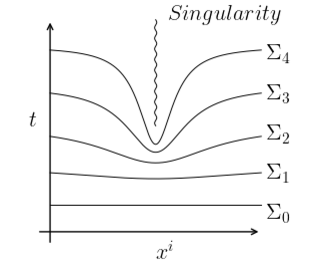
\includegraphics[width=0.4\textwidth]{foliation.png}
%\end{wrapfigure}
Maximal slicing can be implemented by forcing $\mathcal{K} = \partial_t \K = 0$ $\forall t$ which requires a slow elliptic solve for $\alpha$ at each timestep. Instead $\alpha$ is promoted to an evolution variable and is evolved along with every other simulation variable. To do this we can pick an algebraic slicing condition of the following type.
\[\L_m \alpha = -\alpha^2 f(\alpha)\K \]
This is used with $f = 2\alpha^{-1}$ in GRChombo giving
\[\L_m \alpha = -2\alpha \K \]
and using normal coordinates $\beta^i=0$ it reduces to 
\[ \alpha = 1+ \ln \gamma\]
which is called 1+log slicing; this is very common in Numerical Relativity codes. In practice 1+log slicing is strongly singularity avoiding reaching $\alpha=0$ before the singularity. This is modified in the CCZ4 scheme to 
\begin{equation}\partial_t \alpha = -2\alpha\left[ \K-2\Theta\right] + \beta^i \partial_i \alpha\end{equation}
which is very similar to before; it should be noted that the advection term is important for black hole simulations.

So far the shift vector $\beta^i$ has been ignored, the simplest choice for it would be $\beta^i=0$. Using 1+log slicing causes great stretching and shearing of $\Sigma_t$ in the neghbourhood of a singularity and choosing $\beta^i=0$ causes this shear to mean neighbouring gridpoints have large differences in field values leading to inaccurate and unstable evolutions. Another negative side effect is that the computational domain can fall inside an event horizon in black hole simulations. To counteract this we want to pick a shift vector that minimises hypersurface shear $\sigma_{ij}$ which can be defined as [ref 1977 smarr and york]
\[ \sigma_{ij}:= \perp^\mu_i \perp^\nu_j \left[\nabla_{(\mu} n_{\nu)}-\frac{1}{3}\gamma^{ab}\nabla_{(a} n_{b)} \gamma_{\mu\nu}\right] \]
where $\sigma_{ij}$ is tracefree corresponding to shearing rather than inflation or expansion. Minimising total shear, $\Sigma$,
\[ \Sigma = \int \sigma_{ij}\sigma^{ij}\sqrt{\gamma}\,\dd x^3\]
with respect to $\beta^i$ leads to an elliptic PDE to be solved for each $\beta^i$ at each time step that minimises shear. 
\[ \delta \Sigma = 0 \rightarrow \D_i\sigma^{ij}=0\]
This is known as the minimal shift condition. As before, promoting $\beta^i$ to be evolution variables is computationally cheaper. A very common choice is to promote the elliptic PDE for $\beta^i$ into a hyperbolic equation via introducing a $\partial_t^2\beta^i$ term and an artificial damping term parameterised by $\eta$. This becomes a damped wave equation and is supposed to transport away any part of $\beta^i$ which does not satisfy $\D_i \sigma^{ij}=0$. This requires Sommerfeld (outgoing wave) boundary conditions. In GRChombo the standard gamma driver shift condition is used.
\begin{align} \partial_t \beta^i &= FB^i\\
 \partial_t B^i &= \partial_t \tilde{\Gamma}^i - \eta B^i\end{align}
Here $F=3/4$ and $\eta=1$ are used in GRChombo.


\section{Mathematical Modelling of Boson Stars}
\subsection{Action}
The Boson Stars considered are a complex Klein Gordon Scalar field, $\varphi$, minimally coupled to gravity. The action is the Einstein Hilbert vacuum action plus the matter action for curved space.
\begin{gather} S = \int_\mathcal{M}\left[\mathcal{L}_{EH} + \mathcal{L}_M\right] \sqrt{-g}\,\dd x^4 \\
 \L_{EH} = \frac{1}{16\pi G}R \\
 \L_{M} =-\frac{1}{2}g^{\mu\nu}\nabla_\mu \varphi^* \nabla_\nu \varphi - \frac{1}{2}V(|\varphi|^2)  \end{gather}
Here $V$ is the Klein-Gordon potential and it's effect on boson stars is discussed in [].
\begin{align}
V &= \frac{m^2 c^2}{\hbar^2 }|\vp|^2 \rightarrow m^2 |\vp|^2\\
V &= \frac{m^2 c^2}{\hbar^2 }|\vp|^2 + \frac{1}{2}\Lambda|\vp|^4 \rightarrow m^2|\vp|^2 + \frac{1}{2}\Lambda|\vp|^4\\
V &= \frac{m^2 c^2}{\hbar^2 }|\vp|^2\left(1-\frac{|\vp|^2}{2\sigma^2}\right)^2 \rightarrow {m^2 }|\vp|^2\left(1-\frac{|\vp|^2}{2\sigma^2}\right)^2
\end{align}
Considering only the $m^2$ term, which corresponds to the squared mass of the particle in the quantum theory, we get a massive wave equation linear in $\varphi$, leading to so called mini Boson stars. Having $\Lambda\neq0$ gives self-interacting stars which have a nonlinear wave equation corresponding to particle creation and annihilation at the quantum level. Finally, equation 3.6 describes the solitonic potential, giving rise to boson stars with compactnesses comparable to neutron stars. 

Varying the action with respect to the metric and scalar field return the Einstein Field equations and the Klein Gordon equation of curved space respectively.
\begin{equation} R_{\mu\nu} - \frac{1}{2}R g_{\mu\nu} =  \frac{8\pi G}{c^4} T_{\mu\nu}  \end{equation}
\begin{equation}  g^{\mu\nu}\nabla_\mu\nabla_\nu \vp = \frac{\partial V}{\partial |\vp|^2}\vp \end{equation}
Collectively these are known as the Einstein-Klein-Gordon (EKG) equations. The definition and boson-specific stress energy tensors are as follows.
\begin{align}  
T_{\mu\nu} :&= -2\frac{\delta \mathcal{L}_{M}}{\delta g^{\mu\nu}}+g_{\mu\nu}\mathcal{L}_M \\
T_{\mu\nu} &= \frac{1}{2}\nabla_{\mu}\varphi^*\nabla_{\nu}\varphi+\frac{1}{2}\nabla_{\nu}\varphi^*\nabla_{\mu}\varphi-\frac{1}{2}g_{\mu\nu}\left[g^{\alpha\beta}\nabla_\alpha\varphi^*\nabla_\beta\varphi + V\right] 
\end{align}
Studying neutron stars requires the fermionic, or ordinary fluid, stress tensor; this is given below.
\[ T^{\mu\nu}_F = \left[\rho c^2+ {P} \right]\frac{u^\mu u^\nu}{c^2} + P g^{\mu\nu} + 2u^{(\mu}q^{\nu)}+\pi^{\mu\nu}\] 
The vanishing of the divergence, $\nabla_\nu T^{\mu\nu}=0 $, returns the highly nonlinear relativistic Navier-Stokes equations of curved space. The viscosity term $\pi^{\mu\nu}$ and heat flux $q^\mu$ are often omitted for simplicity. The remaining variables $\rho$, $P$ and $u^\mu$ are the fluid density [and enthalpy?], pressure and worldline tangent. Note here the use of sophisticated shock capturing schemes are required, unlike the linear Klein-Gordon equation.


\subsection{Solitons}
A soliton is a wave that exhibits particle-like behaviour. More precisely, in classical field theory, a soliton is a field or set of fields in a localised configuration that can travel at constant speed but not disperse. Some examples of solitons in General Relativity are fluid stars, black holes, wormholes and exotic stars [refernece]. [check are they solitons if they cannot pass though each other (e.g. black holes ...)]. For our purposes, we look for solitons in the Einstein-Klein Gordon (EKG) system which are localised scalar field configurations with accompanying metric. In the case of the real scalar field it was shown by [] that there are no long lived stars; however promoting the field to a complex scalar we can find a spherically symmetric stationary soliton with the following scalar field.
$$ x^\mu \in \{t,r,\theta,\phi \}$$
\begin{equation} \varphi = \Phi(r)e^{i\omega t} \end{equation}
Traditionally, the polar areal gauge has been used [] for the metric's ansatz.
\[g_{\mu\nu}\dd x^\mu \dd x^\nu =- a^2(r)\dd t^2 + b^2(r) \dd r^2 + r^2 \left[ \dd \theta^2 + \sin^2\theta \dd \phi^2\right]\]
The boundary condition $b^2(0)=1$ is demanded to avoid a conical singularity at the origin. However an isotropic gauge is more useful for simulations due to easier conversion to cartesian space-coordinates. The polar areal solution must then be transformed into an isotropic solution. Alternatively, the approach taken in this report, is to start with an isotropic ansatz
\[ g_{\mu\nu}\dd x^\mu \dd x^\nu =- \Omega^2(r)\dd t^2 + \Psi^2(r)\dd \bm{x}^2\]
where $\dd \bm{x}^2$ denotes the euclidean 3D line element; this changes between spherical polar or cartesian coordinates trivially. This ends up being slightly harder to integrate numerically, but no conversion to isotropic coordinates is needed afterwards.

To get a set of ODE's to solve for the functions $\{\Omega(r), \Psi(r),\Phi(r)\}$ we must turn to the Einstein Equation and Klein Gordon Equation. The Einstein Equations for $\{\mu,\nu\}=\{0,0\},\{1,1\},\{2,2\}$ are the only components that give unique non-zero equations; they are given below.
\begin{gather}
\frac{\Omega ^2 \left[r \Psi '^2-2 \Psi  \left[r \Psi ''+2 \Psi '\right]\right]}{r \Psi ^4} = 4\pi G \left[\Omega ^2 \left[\frac{P'^2}{\Psi ^2}+V\right]+\omega ^2 P^2\right]\\
\frac{2 \Psi  \Psi ' \left[r \Omega '+\Omega \right]+r \Omega  \Psi '^2+2 \Psi ^2 \Omega
   '}{r \Psi ^2 \Omega } = 4\pi G \left[P'^2-\Psi ^2 V+\frac{\omega ^2 P^2 \Psi ^2}{\Omega
   ^2}\right]\\
   r \left[-\frac{r \Psi '^2}{\Psi ^2}+\frac{r \Psi ''+\Psi '}{\Psi }+\frac{r \Omega ''+\Omega
   '}{\Omega }\right] = -4\pi G r^2 \Psi ^2 \left[\frac{P'^2}{\Psi ^2}+V-\frac{\omega ^2 P^2}{\Omega
   ^2}\right]
   \end{gather}
  The Einstein tensor $G_{\mu\nu} = R_{\mu\nu}-\frac{1}{2}R g_{\mu\nu}$ (left above) and the stress tensor (right above) were obtained with a self written Mathematica notebook. The Klein Gordon equation (3.6) becomes
  \begin{gather*} \frac{1}{\sqrt{-g}}\partial_\mu \left[ \sqrt{-g}g^{\mu\nu}\partial_\nu \Phi(r)e^{i\omega t}\right] = \frac{\partial V}{\partial |\vp|^2} \Phi(r)e^{i\omega t} \\
  \Phi'' = \Phi\Psi^2\left[V'-\frac{\omega^2}{\Omega^2}\right] - \Phi'\left[\frac{\Omega'}{\Omega} +\frac{\Psi'}{\Psi}+\frac{2}{r} \right]\end{gather*}
Simplifying the Einstein Equations and combinig with the Klein Gordon equation we get 3 ODE's to solve.
\begin{gather}\Omega '=\frac{\Omega}{r\Psi'+\Psi}\left[2 \pi  G r \Psi \left[\Phi'^2 -\Psi^2 
   V+\frac{\omega ^2 \Phi^2 \Psi^2}{\Omega^2} \right]  -\Psi '-\frac{r \Psi '^2}{2 \Psi} \right]
\\{ \Psi'' = \frac{\Psi'^2}{2\Psi} - \frac{2\Psi'}{r}-2\pi G \left[V \Psi^3 + \Phi'^2\Psi+ \frac{ \omega^2\Phi^2\Psi^3}{\Omega^2}\right] }
\\ \Phi'' = \Phi\Psi^2\left[V'-\frac{\omega^2}{\Omega^2}\right] - \Phi'\left[\frac{\Omega'}{\Omega} +\frac{\Psi'}{\Psi}+\frac{2}{r} \right]\end{gather}
This is turned into a set of five first order ODE's to numerically integrate. Note that if we had used the polar areal ansatz () the equation for $\Phi$ would also be first order; reducing the EKG system to four first order ODE's.

\subsection{3+1 Klein Gordon System}
Now let's project the Klein Gordon equation in a 3+1 split to get an evolution equation. The first step is to turn the second order (in time) differential equation into two first order ones
\[ \L_m \{\vp,\Pi \} = ...\]
where $\Pi$ is the foliation dependant definition of conjugate momentum to the complex scalar field.
\begin{equation} \Pi:= -\L_n \vp\end{equation}
Now decompose the Klein Gordon Equation.
\[ \nabla^\mu \nabla_\mu \vp = V' \vp = \frac{1}{\sqrt{-g}} \partial_\mu \left[ \sqrt{-g}\left[\gamma^{\mu\nu}-n^\mu n^\nu\right]\partial_\nu \vp\right] = \frac{1}{\sqrt{-g}} \partial_\mu \left[ \sqrt{-g}\left[\D^\mu\vp-n^\mu \L_n\vp\right]\right] \]
The term with $\D^\mu$ simplifies like
\[\frac{1}{\sqrt{-g}} \partial_\mu \left[ \sqrt{-g}\D^\mu\vp\right] =  \frac{1}{\alpha\sqrt{\gamma}} \partial_\mu \left[\alpha\sqrt{\gamma}\D^\mu\vp\right]  = \D_\mu \D^\mu \vp + \D^\mu \vp \,\partial_\mu \ln \alpha\]
and the remainder becomes
\[-\frac{1}{\sqrt{-g}} \partial_\mu \left[ \sqrt{-g}n^\mu \L_n\vp\right] = -\left[\nabla \cdot n + n\cdot \partial\right]\L_n\vp = -\K\Pi + \L_n \Pi\]
then the full Klein Gordon system is constructed.
\begin{align}
 \L_m \Pi &= - \D^\mu\vp\,\partial_\mu \alpha+\alpha\left[\K\Pi - \D_\mu \D^\mu \vp  + V'\vp\right] \\
 \L_m \vp &= - \alpha\Pi\end{align}
The final matter term we must decompose is the Klein-Gordon stress tensor with equations (). \begin{align} E &=n^\mu n^\nu T_{\mu\nu} = \frac{1}{2}|\Pi|^2 + \frac{1}{2}\gamma^{ij}\D_i \varphi^* \D_j \varphi +\frac{1}{2}V(|\varphi|^2)
\\ S_i &= -\perp^\mu_i n^\nu T_{\mu\nu} =  \frac{1}{2}\left[\Pi^* \D_i \vp  +  \Pi\D_i \vp^* \right]
\\ S_{ij} &= \perp^\mu_i \perp^\nu_j T_{\mu\nu} = \D_{(i}\vp\D_{j)}\vp^* - \frac{1}{2}\left[ \gamma^{ij}\D_i\vp\D_j\vp^* - |\Pi|^2 + V(|\vp|^2)\right]\end{align}

\subsection{Klein Gordon's Noether Charge}
For the complex scalar field, we have the U(1) symmetry
\[\vp \rightarrow \vp e^{i\epsilon} \approx \vp + i\epsilon \vp , \quad\vp^* \rightarrow \vp^* e^{-i\epsilon}  \approx \vp^* - i\epsilon \vp*.\]
This leaves the Lagrangian unchanged and therefore the total action. The associated conserved current $j$ and current density $\mathcal{J}$ are then
\begin{align*} j^\mu &= \frac{\delta \L}{\delta \nabla_\mu\vp}\delta \vp + \frac{\delta \L}{\delta \nabla_\mu \vp^*}\delta \vp*, \quad \nabla_\mu j^\mu =0,\\
 j^\mu &=  ig^{\mu\nu}\left[\vp\nabla_\nu\vp^* - \vp^*\nabla_\nu\vp\right], \quad \mathcal{J}^\mu = \sqrt{-g}j^\mu.\end{align*}
The total integral over a manifold $\M$ gives a conserved charge $\mathcal{Q}$ associated with the conserved current $J^\mu$, assuming $\mathcal{J}^i\rightarrow0$ sufficiently fast towards the boundary $\partial \Sigma_t$ of $\Sigma$.
\[\int_\M \left[\nabla \cdot j\right] \star 1 = 0 = \int_{\phi(\M)} \nabla_\mu j^\mu \sqrt{-g}\,\dd x^4 = \int_{\phi(\M)} \partial_\mu \left[\sqrt{-g} j^{\mu} \right] \dd x^4= \int_{\phi(\M)}\partial_\mu \mathcal{J}^\mu \dd x^4\]
\[ \int^{t_1}_{t_0}\left[\int_{\phi(\Sigma_t)} \partial_0 \mathcal{J}^0 \dd x^3 \right]\dd t = -\int^{t_1}_{t_0}\left[\int_{\phi(\Sigma_t)} \partial_i \mathcal{J}^i \dd x^3 \right]\dd t = 0\]
The term containing $\partial_i\mathcal{J}^i$ integrates to zero over $\Sigma_t$ due to the divergence theorem. The left hand term can be simplified by permuting the time derivative using
\[ \partial_0 \int_{\phi(\Sigma_t)}\mathcal{J}^0 \dd x^3 = \int_{\phi(\Sigma_t)}\partial_0 \mathcal{J}^0 \dd x^3 + \lim_{\Delta x^0\rightarrow0}\left[ \frac{1}{\Delta x^0}\int_{\phi(\Delta \Sigma_t)}\left[ \mathcal{J}^0 +\Delta x^0 \partial_0 \mathcal{J}^0\right] \dd x^3 \right]\]
where the last term vanishes as $\mathcal{J}$ vanishes near $\partial\Sigma$, and we get a formula for the conserved charge.
\[ \partial_0 \int \mathcal{Q}=0, \quad \mathcal{Q} = \int_{\phi(\Sigma_t)}\mathcal{J}^0 \dd x^3 \]
Finally we get an expression for the total Noether charge $\mathcal{N} = \mathcal{Q}[\vp]$
\[\mathcal{N} =i \int_{\Sigma_t} \sqrt{-g}\left[ \vp \nabla^0 \vp^* - \vp^*\nabla^0 \vp\right] \dd x^3\]
and using $\sqrt{-g} = \alpha \sqrt{\gamma}$, $n_\mu \nabla^\mu = -\alpha \nabla^0$ we get the following neat formula.
\begin{equation} \mathcal{N} = i\int_{\Sigma_t}\left[ \vp \Pi^*-\vp^*\Pi\right] \sqrt{\gamma}\,\dd x^3\end{equation}

\subsection{Boosted Boson Stars and Black Holes}
Let us now consider a moving star, this corresponds to making a stationary soliton and boosting it. There is no unique way of doing this as any coordinate transformation that reduces to a Minkowski spacetime boost at large radius will do the job. All the degrees of freedom we have can be absorbed into a coordinate gauge choice, so it makes sense to choose the trivial boost, with rapidity $\chi$, from Special Relativity.
\[\chi=\mathrm{arctanh} \frac{v}{c}\]
\[\Lambda_\nu^\mu =  \exp\begin{pmatrix} 0 & -\chi & 0& 0 \\ -\chi & 0 & 0 & 0\\ 0 & 0&1&0 \\ 0&0&0&1\end{pmatrix} = \begin{pmatrix} \cosh(\chi) & -\sinh(\chi) & 0& 0 \\ -\sinh(\chi) & \cosh(\chi) & 0 & 0\\ 0 & 0&1&0 \\ 0&0&0&1\end{pmatrix} \]
\[\tilde{x}^\mu = \Lambda_{\nu}^{\mu}x^{\nu}\quad \& \quad \tilde{g}_{\mu\nu} = [\Lambda^{-1}]^\alpha_\mu[\Lambda^{-1}]^\beta_\nu g_{\alpha\beta}(\tilde{x}) \]
Declaring the rest and boosted frame to have coordinates $x^\mu$ and $\tilde{x}^\mu$ we choose the boosted soliton's initial Cauchy surface to be the level set of $\tilde{t}=0$. The coordinates and metric transform as follows.
\begin{align*} x^\mu &= \{ t,x,y,z\} = \{\tilde{t}\cosh(\chi) + \tilde{x} \sinh(\chi),\tilde{x}\cosh(\chi)+\tilde{t}\sinh(\chi),\tilde{y},\tilde{z}\} \\
 g_{\mu\nu} &= \mathrm{diag} \{ -\Omega^2, \Psi^2,  \Psi^2, \Psi^2\} \\
 \tilde{g}_{\mu\nu}&=\begin{pmatrix} -\Omega^2\cosh^2 (\chi) + \Psi^2 \sinh^2 (\chi) & \sinh(\chi)\cosh(\chi)\left[\Omega^2-\Psi^2\right] & 0& 0 \\  \sinh(\chi)\cosh(\chi)\left[\Omega^2-\Psi^2\right] & \Psi^2 \cosh^2 (\chi) - \Omega^2 \sinh^2 (\chi) & 0 & 0\\ 0 & 0&\Psi^2&0 \\ 0&0&0&\Psi^2\end{pmatrix}\end{align*}
Comparing this boosted metric to the $3+1$ decomposed metric () we can read off the shift vector $\tilde{\beta}_i$, the 3 metric $\tilde{\gamma}_{ij}$ and obtain the lapse and metric determinant.
\begin{equation} \tilde{\alpha}^2 = \frac{\Psi ^2 \Omega ^2}{\Psi ^2 \cosh ^2(\chi) -\Omega ^2 \sinh ^2(\chi) } \end{equation}
\begin{equation}\tilde{\gamma} = \det \tilde{\gamma}_{ij} = \Psi^4\left[ \Psi^2 \cosh^2 (\chi) - \Omega^2 \sinh^2(\chi)\right]\end{equation}
Finally, the conformal 3-metric with unit determinant is 
\begin{equation} \bar{\gamma}_{ij} = \tilde{\gamma}^{-\frac{1}{3}}\left(
\begin{array}{ccc}
 \Psi ^2 \cosh ^2(\chi) -\Omega ^2 \sinh ^2(\chi)  & 0 & 0 \\
 0 & \Psi ^2 & 0 \\
 0 & 0 & \Psi ^2 \\
\end{array}
\right).\end{equation}
Note normally $\tilde{\gamma}_{ij}$ is the conformal 3-metric, but to avoid confusion with the boosted frame it is denoted $\bar{\gamma}_{ij}$. Turning our attention to the matter fields now we only need to change the coordinate dependance, like $\vp(x)\rightarrow \vp(\tilde{x})$, and remembering $\tilde{t}=0$ defines our boosted frame, which implies $t = \tilde{x}\sinh(\chi)$, we get the following boosted complex scalar field.
\begin{equation}\vp = \Phi(\tilde{x}^2\cosh^2(\chi) +\tilde{y}^2 + \tilde{z}^2)e^{i\omega \tilde{x}\sinh(\chi)} \end{equation}
Note the field is modulated by an oscillatory phase now with wavenumber $k = \omega \tilde{x} \sinh(\chi)$; nodal planes in $\Re(\vp)$ appear perpendicular to velocity. The conjugate momentum $\tilde{\Pi}$ () in the boosted frame it becomes 
\[ \tilde{\Pi}(\tilde{x}^\mu) = -\L_{\tilde{n}} \vp(\tilde{x}^\mu)=-\frac{1}{\tilde{\alpha}}\tilde{m}\cdot \tilde{\partial}\vp = -\frac{1}{\tilde{\alpha}}\left[ \tilde{\partial}_0 - \tilde{\beta}^i\tilde{\partial}_{i}\right]\Phi(r)e^{i\omega t}.\]
Inconveniently we cannot simply evaluate $\tilde{\Pi}$ in the rest frame as this has a different spacetime foliation and the normal vector $n\neq \tilde{n}$ is genuinely changed; not just transforming components under coordinate transformation. Explicitly writing the contravariant components of the shift vector 
\[ \tilde{\beta}^i = \left(\frac{\sinh (\chi)  \cosh (\chi)  \left[\Omega ^2-\Psi ^2\right]}{\Psi ^2 \cosh
   ^2(\chi) -\Omega ^2 \sinh ^2(\chi) },0,0\right)\]
and the partial derivatives of $\vp$ in the boosted frame
\[ \tilde{\partial}_{0} = \cosh(\chi) \partial_t + \sinh(\chi) \partial_x,\quad 
\tilde{\partial}_{1} = \cosh(\chi) \partial_x + \sinh(\chi) \partial_t\] 
 \[\partial_t\vp =\Phi\partial_te^{i\omega t} =i\omega \Phi e^{i\omega t},\quad
 \partial_x\vp =\frac{\partial r}{\partial x}\Phi'e^{i\omega t} = \frac{x}{r}\Phi'e^{i\omega t} \]
we get an expression for the boosted conjugate momentum; explicitly setting $\tilde{t}=0$ gives the momentum on the surface $\tilde{t}=0$ to be used as initial conditions in GRChombo. 
\begin{equation} \widetilde{\Pi} = -\frac{1}{\tilde{\alpha}}\left[  \left[ \sinh(\chi)-\tilde{\beta}^1 \cosh(\chi)\right]\frac{\tilde{x}\cosh(\chi)}{r}\Phi' + i\omega \left[ \cosh(\chi)-\tilde{\beta}^1\sinh(\chi)\right]\Phi\right]e^{i\omega \tilde{x}\sinh(\chi)}\end{equation}
Our final ingredient is the intrinsic curvature, defined in ().
\[ \widetilde{\K}_{\mu\nu} := -\frac{1}{2}\L_{\tilde{n}}\tilde{\gamma}_{\mu\nu} =-\frac{1}{2\tilde{\alpha}}\L_{\tilde{m}}\tilde{\gamma}_{\mu\nu} = -\frac{1}{2\tilde{\alpha}}\left[ \tilde m \cdot \tilde{\partial}\tilde{\gamma}_{ij} +  \tilde{\gamma}_{ik}\tilde{\partial}_j \tilde{m}^k +\tilde{\gamma}_{jk}\tilde{\partial}_i \tilde{m}^k\right]\]
A self written mathematica script gives the following expansion.
\begin{align}\alpha^{-1} \widetilde{\K}_{xx} &= \cosh^2(\chi)\sinh(\chi)\frac{x \left[v^2 \Omega^2 \Omega'+\Psi \Omega \Psi'-2 \Psi^2 \Omega'\right]}{r \Psi^2 \Omega}\\
 \alpha^{-1} \widetilde{\K}_{xy} &= \cosh(\chi)\sinh(\chi)\frac{ y \left[\Omega \Psi'- \Psi \Omega'\right]}{r \Psi \Omega }\\
 \alpha^{-1} \widetilde{\K}_{xz} &= \cosh(\chi)\sinh(\chi)\frac{ z \left[\Omega \Psi'- \Psi \Omega'\right]}{r \Psi \Omega }\\
 \alpha^{-1} \widetilde{\K}_{yy} &= -\sinh(\chi)\frac{ x \Psi'}{ r \Psi }\\
\widetilde{\K}_{zz}&=\widetilde{\K}_{yy} \end{align}
Clearly we can apply this to the Black Hole spacetime by an identical procedure, but ignoring $\vp$ and $\Pi$ and setting the isotropic solutions
\[ \Omega = \frac{1-\frac{M}{2r}}{1+\frac{M}{2r}}, \quad  \quad \Psi = \left[1+\frac{M}{2r}\right]^2.\]
 
 \subsection{Spherical Harmonics in Curved Space}
 Spherical harmonics are an orthonormal function basis for the surface of a sphere. They arise when looking for solutions to the 3D spherical polar laplacian
 \[ \nabla^2 \vp= \frac{1}{\sqrt{|g|}}\partial_{\mu}\left( \sqrt{|g|}g^{\mu\nu}\partial_\nu \vp\right), \quad \mu,\nu \in \{1,2,3\} .\]
 On the hypersurface $r=1$ we get the following metric
 \[ g_{\mu\nu} = \begin{pmatrix} 1 & 0 \\ 0 & \sin^2 \theta\end{pmatrix},\]
 and on this surface the spherical harmonics $Y_{lm}(\theta,\phi)$ satisfy the following condition.
 \[ \D_\mu \D^\mu Y_{lm}(\theta,\phi) = -l(l+1)Y_{lm}(\theta,\phi), \quad x^\mu \in \{\theta,\phi\}\] 
 This means we can take any spherically symmetric and static metric with $g_{\phi\phi} = \sin^2\theta g_{\theta\theta}$ and replace the angular part of the wave equation with $l(l+1)$. For a spherically symmetric spacetime this gives the Klein Gordon equation for scalar hair.
 \[ \nabla_\mu \nabla^\mu \vp = V' \vp, \quad \vp = T(t)R(r)Y_{lm}(\theta,\phi)\]
 \[\vp^{-1}\nabla_\mu \nabla^\mu \vp = g^{tt}\frac{\ddot{T}}{T} +  \frac{1}{R\sqrt{|g|}}\partial_{r}\left( \sqrt{|g|}g^{rr}\partial_r R\right) -{l(l+1)}g^{\theta\theta} \]
 This is a second order ODE for the radial profile $R$ and is an eigenvalue problem for $\omega$ if we assume $T=e^{i\omega t}$. Assuming $T=e^{-kt}$ can be done on-top of the black hole metric () and requires the assumption of no back reaction of the scalar field on the metric; this gives an eigenvalue problem in $k$ instead. This leads to the following ODE for the radial profile. 
 \begin{equation} \frac{1}{R\sqrt{|g|}}\partial_{r}\left( \sqrt{|g|}\Psi^{-4}\partial_r R\right)  = k^2 \frac{\Omega^2}{\Psi^2} + \frac{l(l+1)}{r^2 \Psi^4} + V'\end{equation}
Simulations shown later involve boson stars of mass $M$ and black holes of mass $M\rightarrow 10M$; these simulations often produce scalar hair about these black holes that is orders of magnitude less massive than the boson stars. In this regime the above equation is assumed relevant.


\section{Boson Star Numerical Simulations}
\subsection{Simulation Units}
GRChombo defaults to geometric units, as described in section (1.2). The scalar field $\vp$ appears in the action as
\[ S = \int_{\M} \left[g^{\mu\nu}\partial_\mu \vp \partial_\nu \vp^* + ... \right]\dd x^4\]
and given $S$ and the metric are dimensionless, dimensional analysis tells us $\vp$ has units of inverse length in natural units, or units of energy. The Klein-Gordon mass $m$
\[ \Box \vp = m^2 \vp\]
can be absorbed into new dimensionless spatial coordinates $\tilde{x}^i = x^i m$ changing the KG equation to the scale invariant form.
\[ \Box \vp = \vp\]
\subsection{GRChombo}
GRChombo [] is a recently developed Numerical Relativity code built on top of Chombo [], a PDE solver with fully adaptive mesh refinement (AMR). The advantage of AMR is that regridding, and subsequently sub-volumes of high resolution, is calculated during runtime. This is especially useful for simulating fluids in GR as they can develop features requiring higher resolution in places a human may not expect making pre-specified mesh refinement hard to use. GRChombo uses the CCZ4 system with 1+log slicing and the Gamma driver shift condition, discussed in sections (). GRChombo also supports vectorisation and parallelisation with OpenMP and MPI making it suitable for use on supercomputer clusters. 

So far I have implemented initial data for a single or binary system of compact objects which can be either a Schwarzschild black hole or a boson star. The initial data uses isotropic coordinates and can be boosted along coordinate axes, but not yet general directions, giving the possibility of single boosted objects, accelerated head on collisions, grazing collisions and inspirals/quasi-orbits. It should be noted that my implementation was built on top of the pre-existing complex scalar field class (written by Miren). The remainder of this section will cover the numerical aspects of my work.

\subsection{Initial Data}
Following on from the EKG ODE's () we now seek to solve them numerically to obtain initial data for a single static boson star. The system can be reduced to a set of five first order ODE's so we have 5 boundary conditions. Intuitively, for a physical star we would like to impose $\Phi(0) = \Phi_c$, $\Phi'(0)=0$, $\Phi(r\rightarrow\infty)\rightarrow0$, $\Omega'(0)=0$, $\Omega(r\rightarrow\infty)\rightarrow1$, $\Psi'(0)=0$ and $\Psi(r\rightarrow\infty)\rightarrow1$ to be regular at the origin and match the Schwarzschild vacuum solution at large radius; however this is 7 boundary conditions. One of these can be removed by asking for asymptotic flatness, $\sqrt{\Psi(\infty)}\left(1+\Omega(\infty)\right)=2$, rather than $\Omega(\infty)=\Psi(\infty)=1$, which is inspired by the isotropic black hole metric. One final point of importance is the frequency $\omega$ turns the Klein-Gordon ODE () into an eigenvalue problem, admitting only discrete values of $\omega$.

The first attempt to find the radial profile $\{\Phi(r),\Omega(r),\Psi(r)\}$ of the boson star was to use a relaxation method as it trivially incorporates the above two-point boundary conditions. The modification of promoting equation () to a second order ODE like \[\Omega''(r) = f(g_{\mu\nu},\partial g_{\mu\nu},\Phi,\partial \Phi)\]
is one way we can get an extra degree of freedom to allow 6 boundary conditions; it also means all the EKG ODE's can be written in a parabolic (heat/diffusion equation like) form
\[ \frac{\partial H}{\partial t}  = \nabla^2 H + f(H,...) \]
by introducing an imaginary time $t$ and solved iteratively via evolving in $t$ to a final state where $\dot{H}=0$ thus solving the ODE; this is a relaxation method. In practice this method did not work well with the eigenvalue problem in $\omega$. Unlike with a shooting method, there was no obvious way of telling whether the guess $\omega$ was bigger or smaller than the correct value. Even if this problem were overcome, numerical solution with relaxation takes far longer than than a simple shooting method, even with Chebychev acceleration [], hence a shooting method was chosen over relaxation.

To find the initial data for a single Boson star, a private c++ script was written using RK4 to integrate the EKG system taking 5 initial conditions, and eigenvalue guess $\omega_0$. 
\[ \{\Phi(0),\Phi'(0),\Psi(0),\Psi'(0),\Omega(0);\omega \} = \{ \Phi_c,0,\Psi_c,0,\Omega_c;\omega_0\}\]
Unfortunately we do not know $\Omega_c$ and $\Psi_c$ apriori, but it turns out that guessing any values, such as $\Omega_c=0.5$ and $\Psi_c=2$, still give a boson star. This will generally result in the following asymptotic metric, for constant $A$ and $B$.
\begin{equation} g_{\mu\nu}(r\rightarrow\infty) \rightarrow \mathrm{diag}(-A^2,B^2,B^2,B^2)\end{equation}
However the eigenvalue $\omega$ must be chosen very carefully. It can be shown [], using asymptotics, that the Klein-Gordon equation has a second solution 
\[\vp_2 \approx r^{-1}\exp[r\sqrt{1-\frac{\omega^2}{m^2}}\,]\]
 which eventually dominates for any numerical integration at large radii. Interval bisection was used to find the best value of $\omega$ to machine precision, and at a radius $r_*$ when the large radius mode is deemed to be growing $(\Phi(r_*)=0$ or $\Phi'(r_*)=0)$ the conditions $\Phi(r>r_*)=\Phi'(r>r_*)=0$ are enforced during integration. This creates a vacuum for $r>r_*$ and the spacetime is pure Schwarzschild. After this point, an exponentially growing stepsize was used to reach radii of order $10^8$ times larger than desired for evolutions and the values $A = \Omega_\infty= \sqrt{-g_{00}}$ and $B=\Psi_{\infty}=\sqrt{g_{ii}}$ can be read off. These values are then used iteratively to improve the initial guesses for the metric functions as such $\Omega_c \rightarrow \Omega_c / \Omega_\infty$ and $\Psi_c \rightarrow \Psi_c / \Psi_\infty$ and the interval bisection for $\omega$ is restarted, but with better initial conditions. This is iterated 5 times which leaves $A=B=1$ to extreme precision and the isotropic boson star is created, requiring a few seconds runtime for a high resolution 200,000 grid-point simulation on a laptop.



  \begin{figure}[H]
  \caption{Boson Star radial profile, Left: Ground state, Right: 1st Excited state}
  \centering
  \subfloat{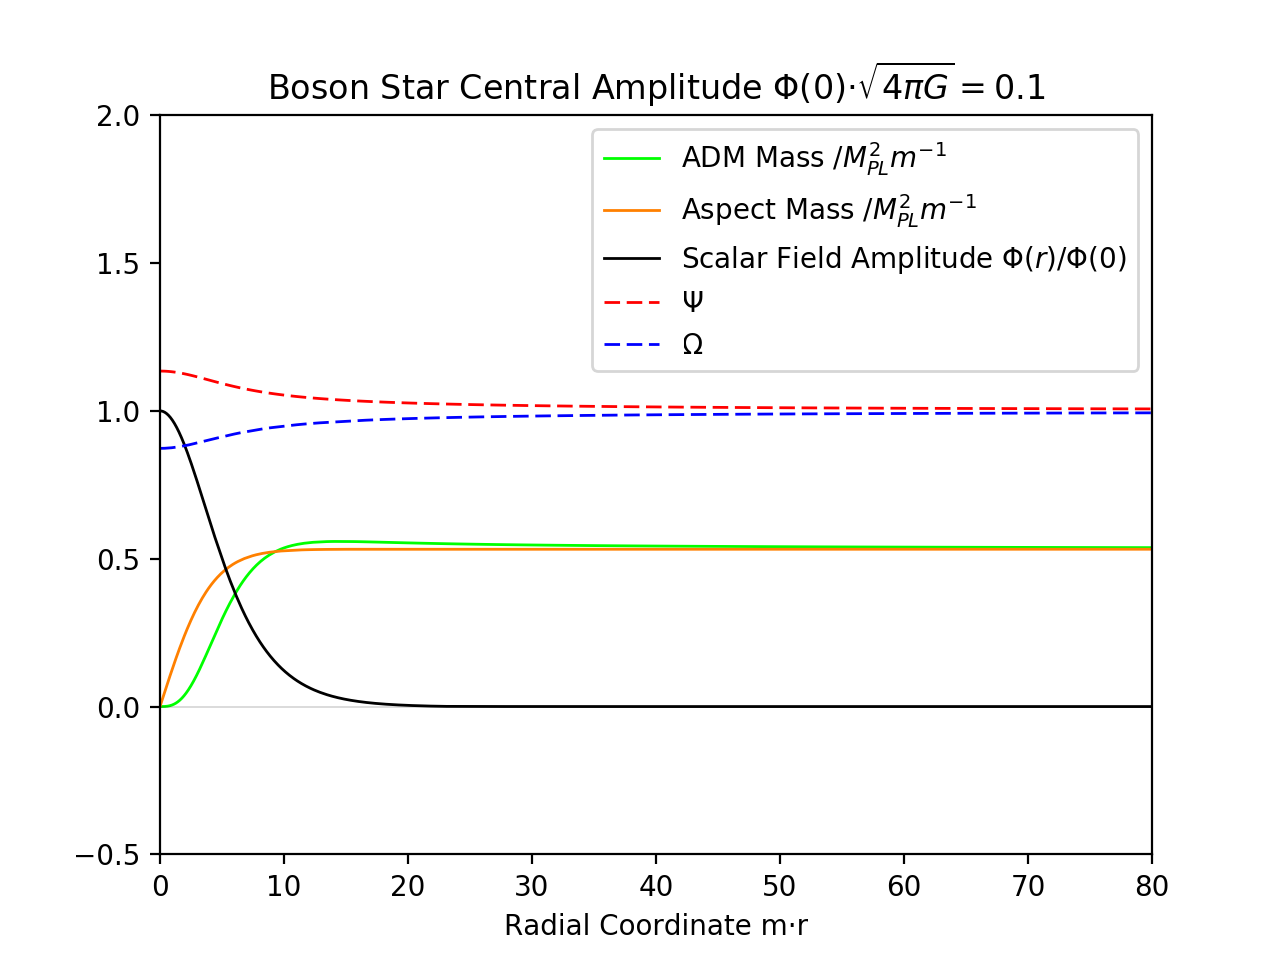
\includegraphics[width=0.5\textwidth]{bosonstar_groundstate.png}\label{fig:f1}}
  \hfill
  \subfloat{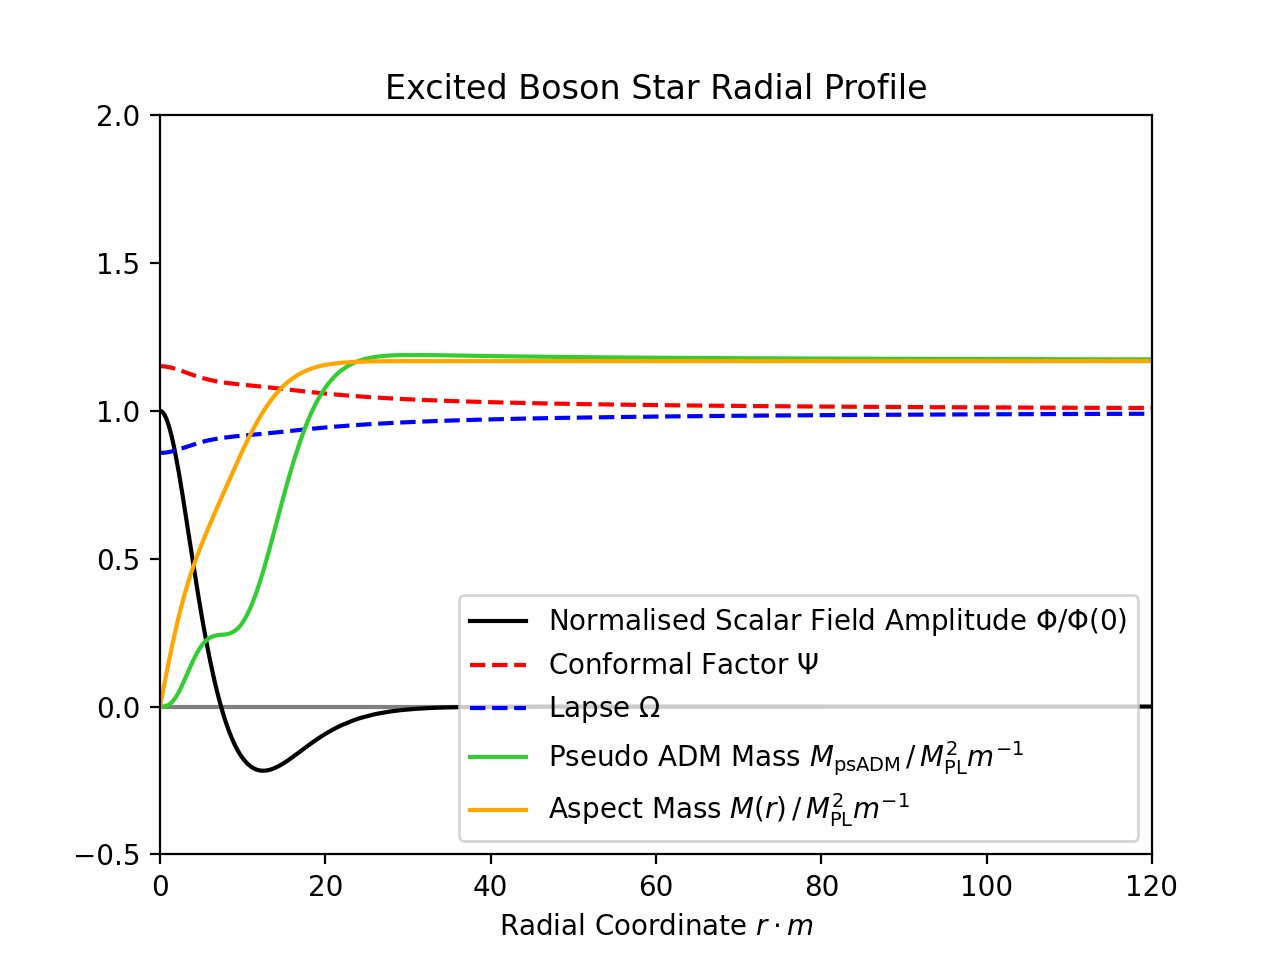
\includegraphics[width=0.5\textwidth]{bosonstar_excitedstate.png}\label{fig:f2}}
\end{figure}

Figures () show the numerical result for the radial profile of a mini boson star ($\Lambda=0$) and an excited mini boson star. Note two mass definitions are plotted; the ADM mass (calculated as a function of finite r) and the aspect mass $M_A(r)$ which corresponds to assuming the metric's solution is Schwarzschild with $M_A(r)$ rather than $M$. Polytropic fluid stars were also simulated as a preliminary test of the code; they are much easier to create not needing to solve an eigenvalue problem and don't have an asymptotically growing mode. Figures () show how the ADM mass of boson stars varies with central amplitude $\Phi(0)$ and $r_{99}$, the radius which $\Phi(r_{99}) = \Phi(0)/100$. It should be noted that the $\Lambda =0$ case agrees with the known maximum mass, the Kaup limit [] $M_{max} \approx 0.633 {M_{PL}^2}{m^{-1}}$ with the highest measured mass being $ M_{max} = 0.63299(3) {M_{PL}^2}{m^{-1}} $ corresponding to a central amplitude of $\ \sqrt{4\pi G}\Phi(0)_{max} = 0.271(0)$. 

  \begin{figure}[H]
  \caption{Boson star trends, Left: ADM mass vs $\Phi(0)$, Right: ADM mass vs $r_{99}$}
  \centering
  \subfloat{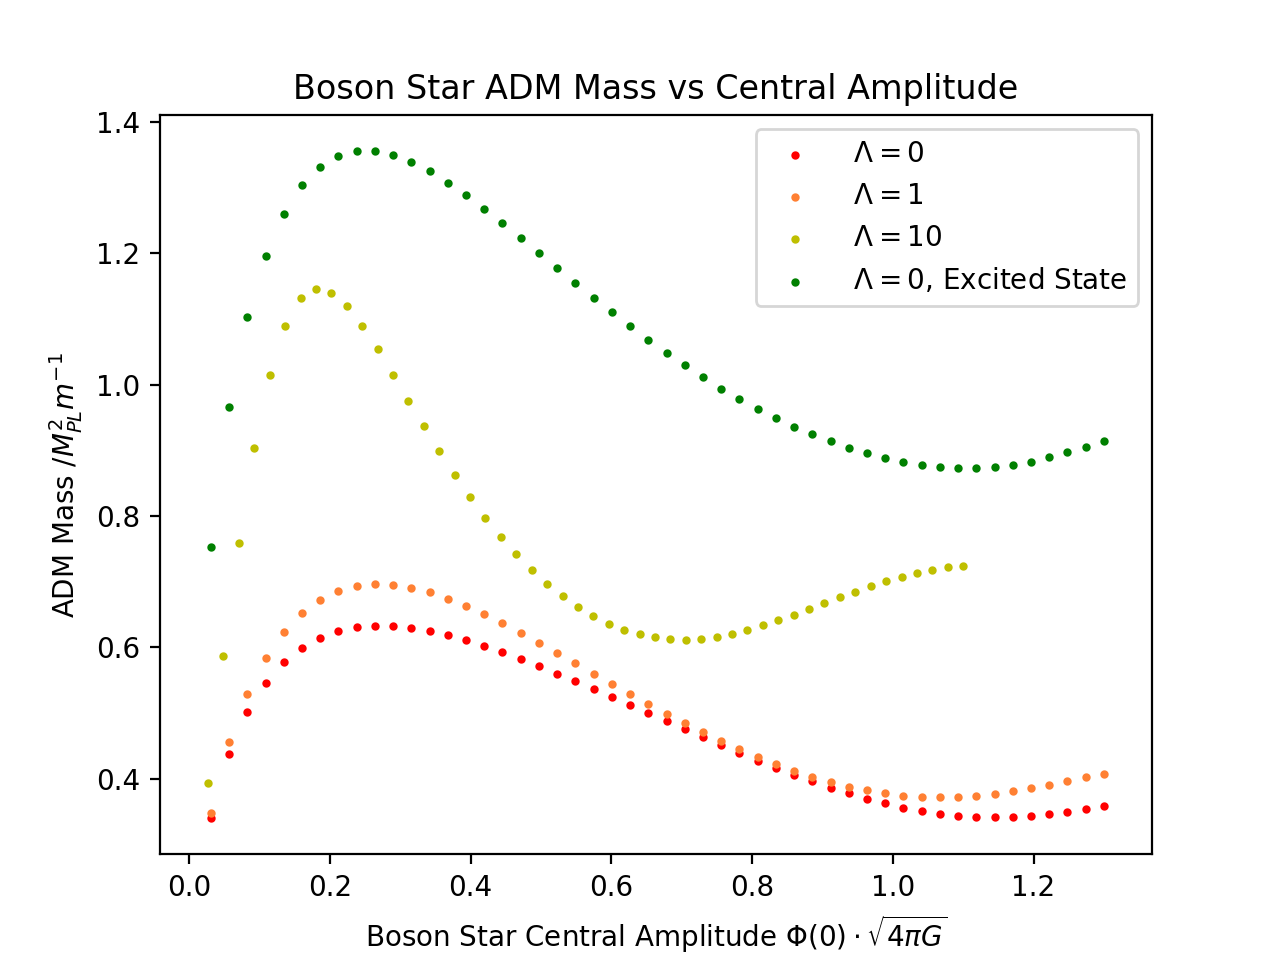
\includegraphics[width=0.5\textwidth]{ADM_vs_PC.png}\label{fig:f1}}
  \hfill
  \subfloat{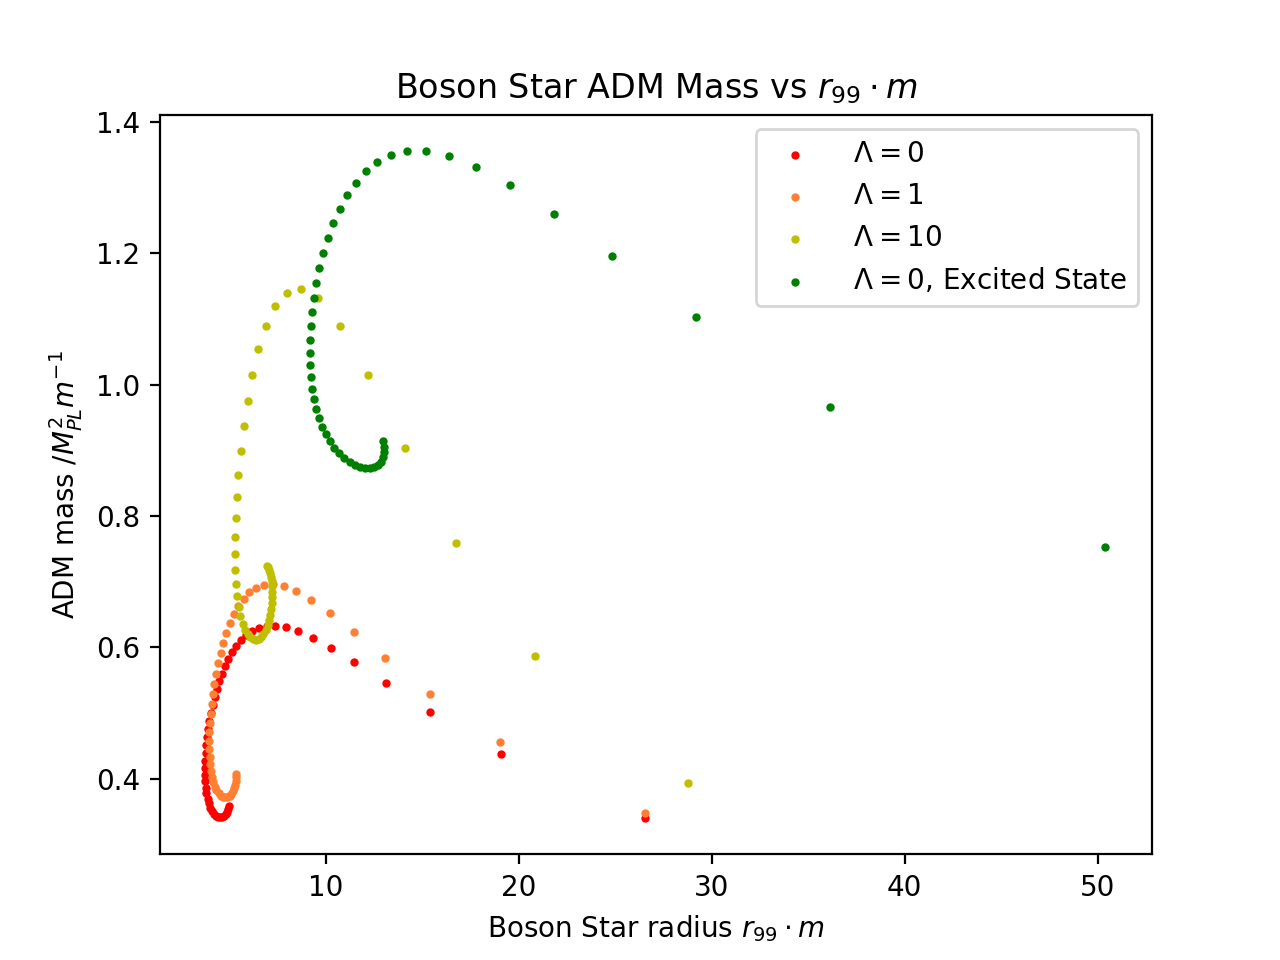
\includegraphics[width=0.5\textwidth]{ADM_vs_r99.png}\label{fig:f2}}
\end{figure}

While many different boson stars have been made to test the initial data code, all the following evolutions use the same boson star with parameters $\Lambda=0$, $\sqrt{4\pi G}\Phi(0)=0.1 \rightarrow \Phi(0) \approx 0.0282$ and ADM mass $M=0.532(7)$. This is as the stars are heavy enough to form black holes under collisions and large deformations, but stable enough to not collapse to a black hole for moderate perturbations.


\subsection{Single Star Evolutions}
  \begin{figure}[H]
  \caption{Left: 2D slice of initial $|\vp|$, Right: Maximum of $|\vp|$ during evolution.}
  \centering
  \subfloat{\includegraphics[width=0.5\textwidth]{mod_phi_nice0000.png}\label{fig:f1}}
  \hfill
  \subfloat{\includegraphics[width=0.5\textwidth]{modphimax.png}\label{fig:f2}}
\end{figure}
The first simulation done was of the $\Phi(0)=0.02820$ mini boson star; as mentioned before all simulations are done with this star. The star is supposed to remain in the centre of the grid and not change as it is a rest frame soliton; this is observed through evolution with GRChombo. Figure () shows a rough initial phase in $|\vp|$ which changes significantly upon changing the AMR regridding, hence it is likely only a side effect of the interpolation errors at the boundary of AMR regions. Figure () shows that the star conserves $\mathcal{N}$ upto 4 figures and the constraint $\mathcal{H}$ is driven towards zero as desired.

  \begin{figure}[H]
  \caption{Left: Total Noether charge $\mathcal{N}$ during evolution, Right: $|| \mathcal{H} ||_2$ during evolution.}
  \centering
  \subfloat{\includegraphics[width=0.5\textwidth]{N.png}\label{fig:f1}}
  \hfill
  \subfloat{\includegraphics[width=0.5\textwidth]{H.png}\label{fig:f2}}
\end{figure}

\subsection{Superposition of Initial Data}
Suppose we have two compact objects with fields $\vp$, $\Pi$, $\gamma_{ij}$, $\K_{ij}$, $\alpha$ and $\beta^i$. The chosen scheme to superpose solutions is below.
\begin{gather*} \vp = \vp^{(1)} + \vp^{(2)}\\
\Pi = \Pi^{(1)} + \Pi^{(2)}\\
 \K^i_j = {\K^{(1)}}^i_j+{\K^{(2)}}^i_j\\
 \gamma_{\mu\nu} = \gamma^{(1)}_{\mu\nu} + \gamma^{(2)}_{\mu\nu}\\
\beta_i = \beta^{(1)}_i + \beta^{(2)}_i \\
 \alpha = \sqrt{\alpha_{(1)}^2 + \alpha_{(2)}^2-1} \quad \mathrm{or}\quad \left[ \alpha_{(1)}^{-1} +  \alpha_{(2)}^{-1}-1\right]^{-1}\\
 \chi = \det{\gamma^{(1)}_{\mu\nu} + \gamma^{(2)}_{\mu\nu}}^{-1/3}\end{gather*}
When a black hole is involved $\Omega(r=\frac{2}{M})=0$ so the event horizon causes the lapse to cross through zero; this is circumvented by setting
\[ \alpha = \sqrt{\chi}\]
and the lapse is real, non-negative for a spacelike hypersurface $\Sigma$. Superposing the scalar field $\vp$ is exact for the mini boson star (); for every other variable and type of star case superposition is inexact. Luckily, for sufficiently separated compact objects, superposition gives a very close approximation to the exact numerical solution. The use of CCZ4 also forces the evolution towards a constraint satisfying one. 



\subsection{Head-on Collisions}
All the cases studied here are for stationary initial data $\tilde{\A}_{ij}=0,\K=0$ in-falling from an initial separation of $d \cdot m = 32$ due to gravitational attraction. Firstly we consider the equal mass Boson star binary, initial data in figure (). At first they slowly infall creating a short lived object with three maxima, shown in figure (,left), then collapse to a black hole with a decaying spherical harmonic cloud (figures ) outside. As with all the simulations from now on we assume a black hole forms if $\chi \ll 16^{-1}$ where $\chi=16^-1$ is the value taken on the horizon for the isotropic Schwarzschild metric.
  \begin{figure}[H]
  \caption{Initial Data, Left: $\chi$, Right: $|\vp|$.}
  \centering
  \subfloat{\includegraphics[width=0.5\textwidth]{headon_bs/chi0000.png}\label{fig:f1}}
  \hfill
  \subfloat{\includegraphics[width=0.5\textwidth]{headon_bs/modphi0000.png}\label{fig:f2}}
\end{figure}
  \begin{figure}[H]
  \caption{Scalar field amplitude before and after black hole formation, Left: Time $t\cdot m = 150$, Right: Time $t \cdot m = 200$.}
  \centering
  \subfloat{\includegraphics[width=0.5\textwidth]{headon_bs/modphi0003.png}\label{fig:f1}}
  \hfill
  \subfloat{\includegraphics[width=0.5\textwidth]{headon_bs/modphi0004.png}\label{fig:f2}}
\end{figure}
   \begin{figure}[H]
  \caption{Real part of scalar field after black hole formation, Left: xy plane, Right: yz plane, perpendicular to initial star separation.}
  \centering
  \subfloat{\includegraphics[width=0.5\textwidth]{headon_bs/phi_re0004.png}\label{fig:f1}}
  \hfill
  \subfloat{\includegraphics[width=0.5\textwidth]{headon_bs/phi_re_perp0004.png}\label{fig:f2}}
\end{figure}
 
The second case considered is the same Boson star outside a black hole parameterised by $M=10M_{BS}$ where $M_{BS}$ is the ADM mass of the Boson star. The scalar field tidally deforms into an ellipsoid with high central density, well beyond Kaup limit of $\vp(0)\sim 0.0764$, and spontaneous collapse to a smaller external black hole is observed. After collapse, figure (), there is an elongated cloud about the new small black hole; there are many nodal lines in $\mathrm{Re}(\vp)$ which focus on the large black hole showing the cloud is in-falling.

  \begin{figure}[H]
  \caption{Initial Data, Left: $\chi$, Right: $|\vp|$.}
  \centering
  \subfloat{\includegraphics[width=0.5\textwidth]{LMR/chi0000.png}\label{fig:f1}}
  \hfill
  \subfloat{\includegraphics[width=0.5\textwidth]{LMR/modphi0000.png}\label{fig:f2}}
\end{figure}
  \begin{figure}[H]
  \caption{Final Data at time $t\cdot m = 125$, Left: Conformal factor $\chi$, Right: Scalar field modulus $|\vp|$, Bottom: Real part of scalarfield $\mathrm{Re}(\vp).$}
  \centering
  \subfloat{\includegraphics[width=0.5\textwidth]{LMR/chi0005.png}\label{fig:f1}}
  \hfill
  \subfloat{\includegraphics[width=0.5\textwidth]{LMR/modphi0005.png}\label{fig:f2}}
  \\
   \subfloat{\includegraphics[width=0.5\textwidth]{LMR/phi_re0000.png}\label{fig:f2}}
\end{figure}
Final case consists of an equal mass Black Hole and Boson Star, initial configuration in Figure 11. As can be seen from the plot of $\Re(\phi)$ and $|\phi|$, in Figure 12, most of the star falls into the black hole, however some scalar field manages to excite an intricate spherical harmonic cloud pattern.
  \begin{figure}[H]
  \caption{Initial data for equal mass Boson Star and Black Hole, Left: $\chi$, Right: $|\vp|$}
  \centering
  \subfloat{\includegraphics[width=0.5\textwidth]{headon/chi0000.png}\label{fig:f1}}
  \hfill
  \subfloat{\includegraphics[width=0.5\textwidth]{headon/mod_phi0000.png}\label{fig:f2}}
\end{figure}
  \begin{figure}[H]
  \caption{Time $t\cdot m=905$ for equal mass Boson Star and Black Hole, Left: $\Re(\vp)$, Right: $|\vp|$}
  \centering
  \subfloat{\includegraphics[width=0.5\textwidth]{headon/phi_re0000.png}\label{fig:f1}}
  \hfill
  \subfloat{\includegraphics[width=0.5\textwidth]{headon/mod_phi0007.png}\label{fig:f2}}
\end{figure}

In all three cases, the Noether charge drops rapidly upon the formation of a black hole; this will be explained in the next section. However some scalar field lingers after collapse, in each case the hair takes the form of spherical harmonics discussed in (). Also observed is the decay of the spherical harmonics to zero amplitude in these simulations with no angular momentum. 
 
\subsection{Binary Inspiral}
The only considered case here is the Quasi-circular orbit and inspiral of two equal mass boson stars. The initial boosts were determined by a newtonian calculation yielding 
\[ v^2 = \frac{M}{2d}\]
where $M=0.53(29)$ is the ADM mass of the Boson Star and d is the initial separation. For a relatively low separation of $d\cdot m =32$ code units, shown in Figures 13,14 (Left), we get $v \sim 0.0915$. The boson stars are observed to complete roughly half an orbit before merging and collapse, forming a black hole. Here a Kerr black hole is assumed to have formed as the spacetime has a significant angular momentum which should partially infall with the scalar field. 

  \begin{figure}[H]
  \caption{Boson Star $|\vp|$. Left: initial data, Right: later time $t \cdot m = 700$}
  \centering
  \subfloat{\includegraphics[width=0.5\textwidth]{inspiral/mod_phi_inspiral_nice0000.png}\label{fig:f1}}
  \hfill
  \subfloat{\includegraphics[width=0.5\textwidth]{inspiral/mod_phi_inspiral_nice0002.png}\label{fig:f2}}
\end{figure}
  \begin{figure}[H]
  \caption{Boson Star $\Re(\vp)$. Left: initial data, Right: later time $t \cdot m = 700$}
  \centering
  \subfloat{\includegraphics[width=0.5\textwidth]{inspiral/phi_inspiral_nice0000.png}\label{fig:f1}}
  \hfill
  \subfloat{\includegraphics[width=0.5\textwidth]{inspiral/phi_inspiral_nice0002.png}\label{fig:f2}}
\end{figure}
  \begin{figure}[H]
  \caption{Left: Total Noether charge $\mathcal{N}$ during evolution, Right: $\Psi_4$ over 22 harmonic during evolution.}
  \centering
  \subfloat{\includegraphics[width=0.5\textwidth]{inspiral/N.png}\label{fig:f1}}
  \hfill
  \subfloat{\includegraphics[width=0.5\textwidth]{inspiral/GW.png}\label{fig:f2}}
\end{figure}
Figure 15 shows the total Noether charge, which is no longer conserved. When the black hole forms, the in-falling scalar field moves towards zero radius and gets hugely compressed. The huge compression causes extreme field gradients which induces continuous regridding in the AMR, but this is capped at 7 layers in this simulation to make runtime feasible. When the 8th AMR level is needed it is simply not added and resolution becomes low enough that any Noether charge near the centre is so under-resolved that it seems to fall between the gridpoints. Interestingly, Figures 13,14 (Right) show a scalar field configuration lingering around the black hole, mostly outside the contour $\chi=0.7$, looking like scalar hair. Also Figure 15 (Left) of the Noether charge appears to take significantly longer to decay than in the linear collision simulations. It can be seen in Figure 14 in the plot of $\Re(\vp)$ that the cloud has angular nodes corresponding to angular momentum similarly to boosted stars picking up nodal planes perpendicular to momentum and Figure 10 (Bottom) of the infalling cloud. 

The gravitational wave (GW) signal can be seen in Figure 15 (Right), extracted at a radius $r \cdot m = 90$. At the time $t \cdot m \approx 700$ the gravitational wave signal due to the merger appears; in order to record a longer inspiral simulations with larger initial separations need to be simulated. Currently there appears to be some small problem with the initial data, also observed in the collisions with no angular momentum, that manifests itself in noisy GW extraction and the Hamiltonian constraint initially sharply rising. 

\section{Future Work}
The first thing that needs to be done is to fix the small error in initial data discussed in section 4.7. After this, the natural extension to work done is to perform binary inspirals with larger radii and inspirals containing an initial black hole. Apart from inspirals, grazing collisions should be studied. A collision with no angular momentum that needs to be looked at is the case of a very small black hole near a large boson star.

Other avenues of study could include exploration of the boson star parameter space, for instance changing central densities, eigenstates, parameters in the potential () and total phase offsets. Binary systems with asymmetric stars are also possible a possibility. 

Finally I plan on studying long lived scalar hair. In general it is difficult to create near extremal Kerr black holes in collisions so it could be useful to create new initial data for this. Maybe collisions with high angular momentum can also produce long lived hair; section 4.7's inspiral shows what appears to be very slowly decaying scalar hair. The study of Proca Stars (spin-1) is another way to study scalar hair and super radiance, here the timescales are often shorter than that for the spin-0 Klein Gordon stars.


